% !TeX program = xelatex
% 中文期刊论文：按照南方电网技术投稿要求改写
% 编译建议：XeLaTeX。中文字体优先使用系统字体，缺失时回退到 TeX Live/CTeX 常见的 Fandol 字体。
\documentclass[UTF8,zihao=5,twoside]{ctexart}

\usepackage[a4paper,top=22mm,bottom=20mm,left=18mm,right=18mm,headheight=14pt,headsep=6mm,columnsep=7mm]{geometry}
\usepackage{fontspec}
\usepackage{xeCJK}
\usepackage{amsmath,amssymb,bm}
\usepackage{graphicx}
\usepackage{float}
\usepackage{booktabs,array,multirow,tabularx}
\usepackage{caption}
\usepackage{titlesec}
\usepackage{fancyhdr}
\usepackage{indentfirst}
\usepackage{enumitem}
\usepackage{multicol}
\usepackage{balance}
\usepackage{tikz}
\usetikzlibrary{arrows.meta,positioning,shapes.geometric}
\usepackage[hidelinks]{hyperref}

\graphicspath{{figures/}}

% -------------------- 字体 --------------------
\IfFontExistsTF{Songti SC}
  {\setCJKmainfont{Songti SC}}
  {\IfFontExistsTF{SimSun}
    {\setCJKmainfont{SimSun}}
    {\setCJKmainfont{FandolSong-Regular.otf}[BoldFont=FandolSong-Bold.otf,ItalicFont=FandolKai-Regular.otf]}}
\IfFontExistsTF{Heiti SC}
  {\setCJKsansfont{Heiti SC}}
  {\IfFontExistsTF{SimHei}
    {\setCJKsansfont{SimHei}}
    {\setCJKsansfont{FandolHei-Regular.otf}[BoldFont=FandolHei-Bold.otf]}}
\IfFontExistsTF{Kaiti SC}
  {\setCJKfamilyfont{kai}{Kaiti SC}}
  {\IfFontExistsTF{KaiTi}
    {\setCJKfamilyfont{kai}{KaiTi}}
    {\setCJKfamilyfont{kai}{FandolKai-Regular.otf}}}
\IfFontExistsTF{Times New Roman}{\setmainfont{Times New Roman}}{\IfFontExistsTF{TeX Gyre Termes}{\setmainfont{TeX Gyre Termes}}{\setmainfont{Latin Modern Roman}}}
\IfFontExistsTF{Arial}{\setsansfont{Arial}}{\IfFontExistsTF{TeX Gyre Heros}{\setsansfont{TeX Gyre Heros}}{\setsansfont{Latin Modern Sans}}}
\newcommand{\kaiti}{\CJKfamily{kai}}

\zihao{5}
\setlength{\parindent}{2em}
\linespread{1.08}
\setlist{nosep,leftmargin=2em}
\setlength{\textfloatsep}{0.7em plus 0.2em minus 0.2em}
\setlength{\floatsep}{0.6em plus 0.2em minus 0.2em}
\setlength{\intextsep}{0.6em plus 0.2em minus 0.2em}
\renewcommand{\topfraction}{0.95}
\renewcommand{\bottomfraction}{0.85}
\renewcommand{\textfraction}{0.05}
\renewcommand{\floatpagefraction}{0.85}
\setcounter{topnumber}{4}
\setcounter{bottomnumber}{2}
\setcounter{totalnumber}{6}

% -------------------- 页眉页脚 --------------------
\pagestyle{fancy}
\fancyhf{}
\fancyhead[LE]{\zihao{-5}第~\thepage~页}
\fancyhead[CE]{\zihao{-5}南方电网技术}
\fancyhead[RE]{\zihao{-5}第~XX~卷}
\fancyhead[LO]{\zihao{-5}\thepage}
\fancyhead[CO]{\zihao{-5}南方电网技术}
\fancyhead[RO]{\zihao{-5}第~XX~卷}
\renewcommand{\headrulewidth}{0.4pt}
\renewcommand{\footrulewidth}{0pt}

% -------------------- 标题层级 --------------------
\titleformat{\section}{\sffamily\zihao{4}\bfseries}{\thesection}{0.6em}{}
\titleformat{\subsection}{\sffamily\zihao{5}\bfseries}{\thesubsection}{0.6em}{}
\titleformat{\subsubsection}{\sffamily\zihao{5}\bfseries}{\thesubsubsection}{0.6em}{}
\titlespacing*{\section}{0pt}{0.8em}{0.4em}
\titlespacing*{\subsection}{0pt}{0.6em}{0.3em}
\titlespacing*{\subsubsection}{0pt}{0.4em}{0.2em}

% -------------------- 图表与公式 --------------------
\captionsetup{font={small},labelfont=bf,labelsep=quad,justification=centering}
\renewcommand{\figurename}{图}
\renewcommand{\tablename}{表}
\numberwithin{equation}{section}
\renewcommand{\theequation}{\arabic{equation}}

\newcommand{\figbicaption}[2]{%
  \caption{#1\\[-0.2em]\small Fig.\,\thefigure\ #2}
}
\newcommand{\tabbicaption}[2]{%
  \caption{#1\\[-0.2em]\small Tab.\,\thetable\ #2}
}
\newcommand{\metric}[1]{\mathrm{#1}}
\newcommand{\code}[1]{\texttt{#1}}

% -------------------- 参考文献格式 --------------------
\renewcommand{\refname}{参考文献}
\makeatletter
\renewenvironment{thebibliography}[1]{%
  \section*{\refname}%
  \small
  \list{[\arabic{enumi}]}{%
    \settowidth\labelwidth{[#1]}%
    \leftmargin\labelwidth
    \advance\leftmargin\labelsep
    \usecounter{enumi}}
  \sloppy\clubpenalty4000\widowpenalty4000\sfcode`\.\ \@m
}{\def\@noitemerr{\@latex@warning{Empty `thebibliography' environment}}\endlist}
\makeatother

\newcommand{\articleinfo}{文章编号：1674-0629(20XX)XX-XXXX-XX\quad 中图分类号：TM73\quad 文献标志码：A\\
DOI：10.13648/j.cnki.issn1674-0629.20XX.XX.XXX}

\newcommand{\fundcn}{基金项目：无。}
\newcommand{\funden}{Foundation item: None.}

\begin{document}
\twocolumn[

% ==================== 首页题名与摘要：单栏 ====================
\begin{center}
{\zihao{-5}\articleinfo}\par\vspace{1.0em}
{\sffamily\zihao{2}\bfseries 基于多相关性筛选与 L1 门控深度神经网络的电力数据隐性推断源定位}\par\vspace{0.8em}
{\zihao{4}杜浩存}\par\vspace{0.4em}
{\zihao{5}（西安交通大学 网络空间安全学院，陕西 西安 710049）}\par\vspace{0.8em}
\end{center}

\noindent\textbf{摘要：}电力系统运行与市场数据由物理约束、调度策略和市场出清机制共同生成，字段之间存在复杂而稳定的统计关联，部分目标字段虽未直接给出，却可能由若干低关注度字段联合恢复，构成隐性推断。针对传统相关性分析难以刻画联合推断能力、全量深度模型难以定位关键推断源字段的问题，提出一种融合多相关性筛选与 L1 门控深度神经网络（deep neural network，DNN）的电力数据隐性推断源定位方法。该方法首先以 Pearson、Spearman、Kendall 相关系数以及归一化互信息、距离相关系数和希尔伯特--施密特独立性准则六类指标对候选字段进行多维依赖性初筛；继而在 DNN 输入端引入可学习门控向量并施加 L1 正则化，压缩冗余字段并获取紧凑的推断源集合；进而构建相关性驱动的改进门控，使门控强度由六类相关性指标统一驱动。基于美国 PJM 电力市场 2025 年小时级运行数据的实验表明：以净实际交换功率为目标，所提方法从 69 个候选字段中定位出 18 个推断源，据此再训练的 DNN 测试决定系数 $R^2$ 达 0.968，高于全量字段的 0.966，而其余 51 个字段单独推断仅为 0.782；在 12 个目标字段上平均使用 15.5 个字段（约占全量的 22.46\%）即取得 0.911 的平均 $R^2$，优于全量模型的 0.903。同预算对比与冗余信息分析进一步验证了所提方法在字段压缩与推断能力保持方面的有效性。\par
\noindent\textbf{关键词：}电力数据；关联性分析；隐性推断源；L1 门控神经网络；特征选择；数据共享\par\vspace{0.8em}

\begin{center}
{\bfseries\large Locating Implicit Inference Sources in Power Data Based on Multi-Correlation Screening and L1-Gated Deep Neural Network}\par\vspace{0.5em}
{DU Haocun}\par\vspace{0.3em}
{\small (School of Cyber Science and Engineering, Xi'an Jiaotong University, Xi'an 710049, China)}\par\vspace{0.5em}
\end{center}

\noindent\textbf{Abstract:} Power system operation and market data are jointly shaped by physical constraints, dispatching strategies and market clearing mechanisms, giving rise to complex and stable statistical dependencies among data fields. Consequently, some target fields that are not directly released may still be jointly recovered from several low-attention fields, constituting implicit inference. To address the limitations of conventional correlation analysis in characterizing joint inference capability and the difficulty of full-feature deep models in locating critical inference-source fields, this paper proposes a method for locating implicit inference sources in power data by integrating multi-correlation screening with an L1-gated deep neural network (DNN). The method first screens candidate fields along multiple dependency dimensions using six measures: Pearson, Spearman and Kendall correlation coefficients, normalized mutual information, distance correlation, and the Hilbert-Schmidt independence criterion. A learnable gate vector is then inserted at the DNN input layer and trained with L1 regularization to compress redundant fields and obtain a compact inference-source set. Furthermore, a correlation-driven improved gate is constructed so that the gating strength is jointly driven by the six correlation measures. Experiments on the 2025 PJM hourly market data show that, for net actual interchange, the proposed method locates 18 inference sources out of 69 candidate fields, and a DNN retrained on them attains a test coefficient of determination $R^2$ of 0.968, higher than 0.966 obtained with all fields, whereas the remaining 51 fields alone yield only 0.782. Across 12 target fields, the method uses 15.5 fields on average (about 22.46\% of all fields) yet achieves an average $R^2$ of 0.911, exceeding 0.903 of the full-feature model. Same-budget baseline comparisons and redundant-information analysis further validate the effectiveness of the proposed method in field compression and inference preservation.\par
\noindent\textbf{Key words:} power data; correlation analysis; implicit inference source; L1-gated neural network; feature selection; data sharing\par\vspace{0.8em}

\noindent{\small\fundcn\\\funden}
\vspace{0.8em}
]

\section{引言}
在大数据时代，信息与量测技术的进步使电网运行中产生了海量电力数据，有效利用这些数据对科学决策与电力系统可持续发展至关重要\cite{ref-liu-cps}。随着新型电力系统建设和电力市场化改革推进，调度运行、市场出清、负荷预测、辅助服务、燃料结构与区域交换等环节不断产生多源、多粒度、高维度的结构化数据\cite{ref-ma-pjm,ref-fan-pjm}。然而，电网由众多互联节点与线路构成、运行机制复杂，且电力数据异构性强、体量庞大、价值分布稀疏，真正有分析价值的信息往往淹没在大量字段之中\cite{ref-xing-micdnn}。

更为重要的是，电力数据与电力行业的业务运营高度交织。电网借助电力系统模型计算生成大量系统数据与量测数据，并在潮流平衡、机组组合、市场报价与调度策略的共同作用下，使不同类型字段之间形成广泛的派生关系与统计耦合，数据类别之间的界限日趋模糊\cite{ref-xing-micdnn}。因此，字段之间往往并非相互独立：某些并未直接发布的目标字段，可能由若干公开或低关注度字段的组合所重构，从而构成隐性推断源。

识别隐性推断源在多种分析场景中均具有现实意义。一方面，在电网运行分析中，研究者常需厘清某一关键运行量（如区域负荷、节点电价或交换功率）的取值与波动主要由哪些因素决定，即在众多量测字段中找出能够重构该量的关键变量，从而为预测建模、异常溯源与运行优化提供依据\cite{ref-deng-load}。另一方面，在数据安全与隐私场景下，电网运行状态量通常被视为具有较高价值，其关联字段数量众多，若不加甄别地共享，公开字段的组合可能被用于反向推断出未直接发布的信息。已有研究将这类由数据关联导致的信息恢复归纳为信息物理系统中的数据推断威胁\cite{ref-liu-inference}，并在智能电表隐私\cite{ref-sankar,ref-giaconi}、能源分解\cite{ref-adewole}以及电力大数据隐私保护\cite{ref-chen-privacy,ref-zhang-sgcc}等方向展开了大量工作。两类场景出发点虽异，却指向同一核心问题：在普遍存在派生与耦合关系的电力数据中，如何刻画并定位对目标字段真正具有推断能力的字段集合。

然而，正因电力数据字段众多、关联路径复杂且彼此耦合，与目标相关的候选字段往往数量庞大且高度冗余，仅凭两两关联难以回答“哪些字段真正构成隐性推断源”。因此在定位之前，必须定量刻画字段的关联强度与推断贡献，并从大量相关字段中剔除冗余、保留不可替代的关键字段。相关性分析是刻画字段间关联的常用手段：Pearson 相关系数、Spearman 和 Kendall 秩相关系数已广泛应用于负荷预测与数据清洗中的特征筛选\cite{ref-lan-load,ref-jiao-pv,ref-deng-load}；为刻画变量间的非线性依赖，距离相关系数\cite{ref-szekely-dcorr}和希尔伯特--施密特独立性准则（Hilbert-Schmidt independence criterion，HSIC）\cite{ref-gretton-hsic}等核方法也被引入电力数据分析。相关性分析计算代价低、结果直观且便于解释，适合在高维字段空间中进行初步筛查；但单一指标只能反映特定数学意义下的两两依赖：线性相关、秩相关、分布依赖与核空间相关所捕获的信息各不相同。在电力数据中，同一目标字段可能同时受到线性耦合、单调非线性关系与复杂市场规则的影响，若仅采用一种指标，易遗漏弱线性但强非线性的潜在推断源。文献\cite{ref-xing-micdnn}提出的 MIC-DNN 框架将最大信息系数（maximal information coefficient，MIC）\cite{ref-reshef-mic}与深度模型相结合用于电力数据关联验证，但该方法侧重成对推断，尚难以在多字段联合场景下识别出既具推断能力又相对非冗余的推断源集合。

基于机器学习的推断建模为验证字段间推断能力提供了另一条途径。深度神经网络\cite{ref-lecun-deep,ref-goodfellow-deep}、随机森林\cite{ref-breiman-rf}和极端梯度提升树（XGBoost）\cite{ref-chen-xgboost}等模型已在电力数据分析中得到广泛应用\cite{ref-wang-meter}，能够直接检验目标字段是否可由其他字段恢复；但全量深度模型通常只给出整体可预测性判断，难以回答“哪些字段构成主要推断源”这一关键问题。Lasso\cite{ref-tibshirani-lasso}和弹性网络（ElasticNet）\cite{ref-zou-enet}等稀疏线性模型虽具备变量选择能力，但其表达能力受限于线性假设；树模型的特征重要性排序则易受特征冗余与训练随机性的干扰。

综上，面向电力数据关联分析的隐性推断源定位需同时处理两个问题：候选字段多导致潜在推断路径难以穷举，以及字段强耦合导致冗余信息需要剔除。初筛过窄会因忽略非线性或互补依赖而漏判，直接以全量字段建模又会引入大量冗余与弱相关字段，既削弱可解释性，也可能掩盖真正支撑目标推断的关键路径。为此，本文构建一种由宽到严的分析流程：先以多类统计依赖证据进行保守初筛，再在非线性推断模型中以稀疏约束压缩冗余字段，最后通过独立再训练与对比实验验证所定位字段集合的实际推断能力。主要贡献如下：

1）构建面向电力运行与市场数据的隐性推断源定位框架，将多相关性初筛、稀疏字段选择与再训练验证组织为统一流程；并在 DNN 输入端引入 L1 门控层，使字段取舍由统计依赖证据与推断误差共同驱动，在保留主要推断路径的同时压缩冗余字段。

2）提出相关性驱动的改进门控模型，将字段的六维相关性向量经线性映射与 Sigmoid 激活转化为门控值，使门控强度由各类相关性指标共同驱动并随推断训练自适应学习，从而为不同指标对推断源判定的贡献提供可解释的量化方式。

3）基于 PJM 2025 年小时级运行与市场数据，开展单目标分析、多目标对比、同预算特征选择对比及冗余信息影响分析，验证所提方法在字段压缩与推断能力保持方面的有效性。

\section{隐性推断源定位方法}
\subsection{问题定义}
给定电力数据集
\begin{equation}
D=\{X_1,X_2,\ldots,X_w,Y\},
\end{equation}
其中 $Y\in\mathbb{R}^{n}$ 为关注的目标字段，$X_i\in\mathbb{R}^{n}$ 为候选字段，$w$ 为候选字段总数，$n$ 为样本数。在数据共享场景中，$Y$ 可表示交换功率、电价、备用容量、负荷或其他具有较高分析价值的字段，$X_i$ 则表示可能被公开或以较低关注度共享的字段。若利用部分 $X_i$ 即可对 $Y$ 建立有效推断模型，则即使 $Y$ 本身未被直接给出，也可能由这些字段联合恢复，从而构成隐性推断源。

本文关注的不是一般意义上的预测精度提升，而是关联分析中的字段级推断源定位问题。其目标是在候选字段中识别一个规模尽可能小的集合 $\mathcal{S}$，使其对目标字段 $Y$ 仍能维持较高推断精度：
\begin{equation}
\mathcal{S}^{*}=\arg\min_{\mathcal{S}\subseteq \{X_i\}}\left|\mathcal{S}\right|,
\quad
R^2(f_{\theta}(\mathcal{S}),Y)\geq \eta .
\end{equation}
式中：$f_{\theta}$ 为推断模型；$\eta$ 为可接受的推断能力阈值。$\mathcal{S}^{*}$ 的规模越小，说明目标字段越可能由少量字段恢复；若 $\mathcal{S}^{*}$ 中的字段具有明确业务含义，则可进一步为字段降精度、延迟发布、合并发布或分级共享等数据处置策略提供依据。模型推断性能采用决定系数 $R^2$ 衡量：
\begin{equation}
R^2=1-\frac{\sum_{k=1}^{n}(y_k-\hat{y}_k)^2}{\sum_{k=1}^{n}(y_k-\bar{y})^2}.
\end{equation}
式中：$y_k$ 为真实值；$\hat{y}_k$ 为模型预测值；$\bar{y}$ 为真实值的均值。当一个规模较小的字段集合所取得的 $R^2$ 接近或超过全量字段时，表明该集合保留了主要推断路径；反之，当被剔除字段单独推断能力显著下降时，则说明这些字段主要贡献冗余信息或噪声。

本文方法的总体流程如图~\ref{fig:method_flow} 所示：先设定目标字段、整理候选字段，计算候选字段与目标之间的六类相关性指标并以宽松规则初筛；继而将初筛字段送入 L1 门控深度推断模型，由预测损失与稀疏惩罚共同学习活跃推断源；最后以普通 DNN 对选中字段再训练验证，并结合门控值与相关性权重解释推断源构成。该流程使初筛、门控压缩与再训练验证分工协作：初筛保证候选覆盖率，门控定位并压缩推断路径，再训练则避免将门控自身的训练偏差误判为字段贡献。

\begin{figure}[!htbp]
\centering
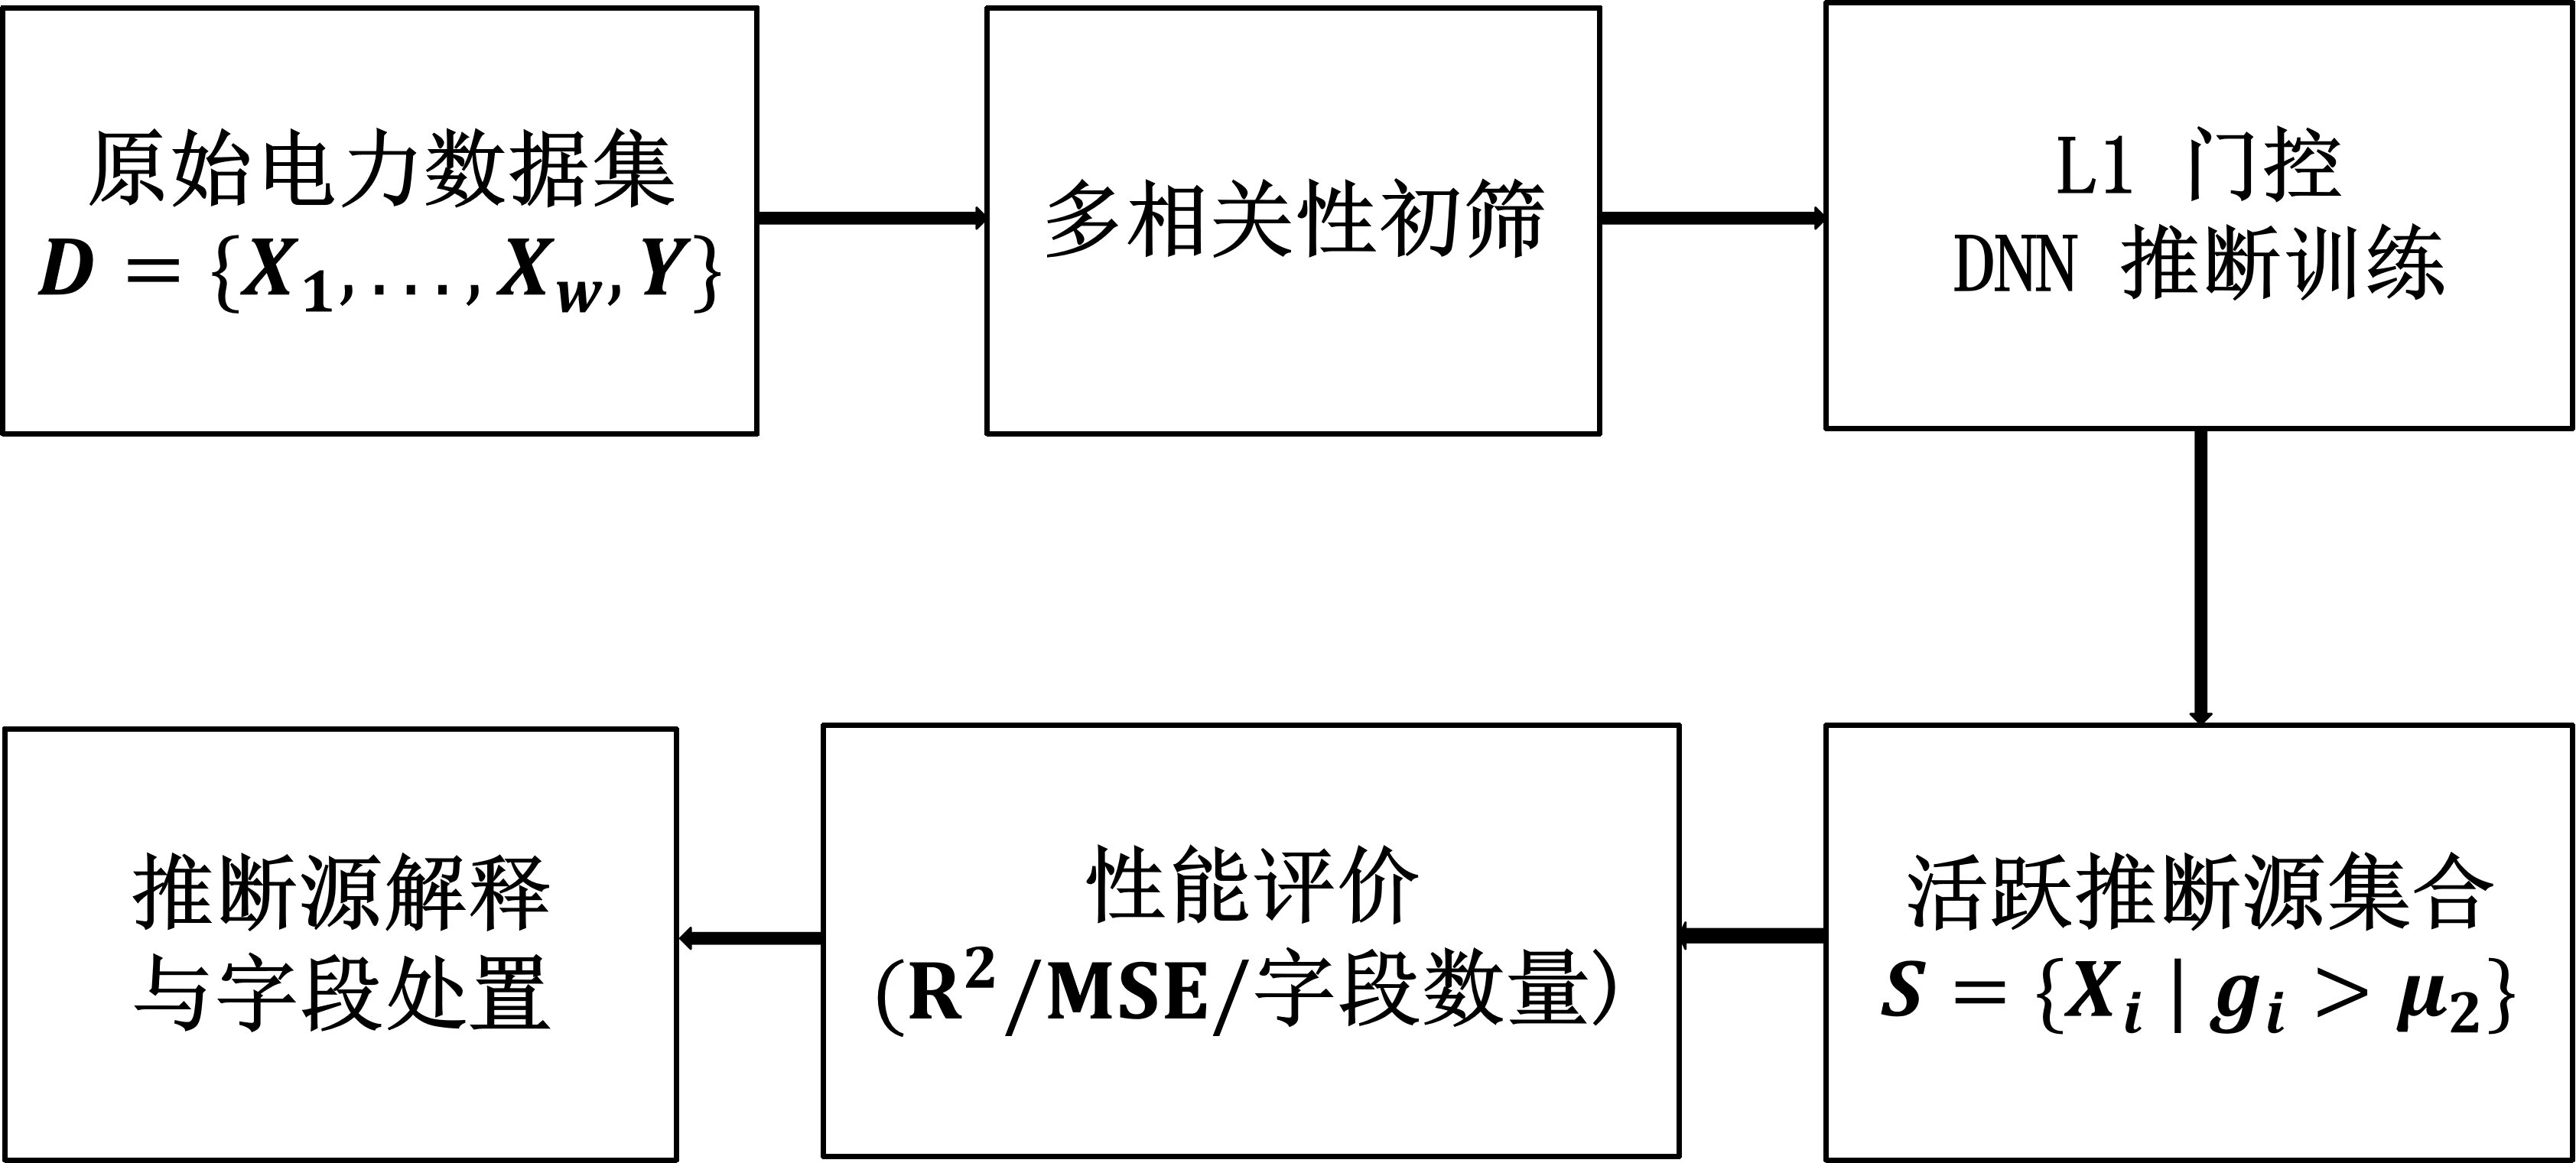
\includegraphics[width=\columnwidth]{总体流程.png}
\figbicaption{隐性推断源定位总体流程}{Overall workflow of implicit inference source localization}
\label{fig:method_flow}
\end{figure}

\subsection{多相关性初筛}
相关系数是刻画变量间关联关系的常用统计工具，其基本思想是将两个变量之间的同步变化程度、排序一致性、分布依赖或核空间依赖压缩为一个可比较的数值。对于高维电力数据的关联分析而言，相关系数具有两个优点：一是计算效率高，可在大量字段上快速执行；二是结果具有较好的可解释性，便于对候选字段进行初步排序和筛查。但是，相关系数本质上属于描述性统计量，只能说明变量之间存在某种关联，不能直接证明某个字段在联合推断模型中不可替代。因此，本文将相关性分析定位为候选空间压缩和推断线索发现，而不是最终的推断源判定。

电力数据字段之间的依赖关系具有多样性：既可能因潮流方程、功率平衡或数据聚合形成近似线性关系，也可能因市场出清机制、辅助服务约束和分段调度规则产生复杂的非线性耦合。为降低单一统计指标造成的漏筛，本文构建六维相关性向量对每个候选字段 $X_i$ 进行综合评估：
\begin{equation}
R_i=[r_i^{(\metric{NMI})},r_i^{(\metric{Spear})},r_i^{(\metric{Pear})},
r_i^{(\metric{Ken})},r_i^{(\metric{DC})},r_i^{(\metric{HSIC})}].
\end{equation}
式中：六个分量分别对应归一化互信息（normalized mutual information，NMI）、Spearman 秩相关系数、Pearson 相关系数、Kendall 秩相关系数、距离相关系数（distance correlation，DC）和希尔伯特--施密特独立性准则（HSIC）。六类指标各有侧重。

Pearson 相关系数度量两个变量之间的线性相关程度，其定义为
\begin{equation}
\rho_{p}(X_i,Y)=
\frac{\mathrm{cov}(X_i,Y)}{\sigma_{X_i}\sigma_Y}.
\end{equation}
当字段之间存在近似线性派生关系或同步波动时，Pearson 系数能够给出直接反映。Spearman 相关系数先将变量转换为秩序列，再计算秩序列的 Pearson 相关，适合刻画单调但非严格线性的关系。Kendall 秩相关系数基于样本对的一致序和逆序关系定义，能够从排序一致性的角度反映变量间关联，对异常值和局部非线性变化相对稳健。

归一化互信息从信息论\cite{ref-cover-info}角度度量变量之间共享的信息量，能够发现非单调和非线性依赖；本文将互信息按变量熵进行归一化，使其落入可比较范围。距离相关系数基于样本间距离矩阵度量变量依赖，当且仅当变量独立时其理论值为 0，因而能够捕捉一般形式的非线性关系。HSIC 则将变量映射到再生核希尔伯特空间中，通过核矩阵的相关性度量统计依赖，适合刻画复杂非线性耦合。本文同时采用上述六类指标，是因为电力数据中线性、单调、非单调和高阶非线性依赖往往并存，任何单一指标都难以覆盖全部潜在推断路径。

初筛流程如图~\ref{fig:screening_flow} 所示。对每个候选字段，先分别计算六类相关性得分，并将不同指标的得分与对应阈值比较；随后采用“任一指标通过即保留”的宽松策略，即当任意一个指标达到预设阈值时，该字段即被保留进入后续门控建模：
\begin{equation}
\max_j I\left(r_i^{(j)}\geq \mu_1^{(j)}\right)>0.
\end{equation}
式中：$I(\cdot)$ 为示性函数；$\mu_1^{(j)}$ 为第 $j$ 类指标的初筛阈值。该策略的设计原则是宁可保留部分弱冗余字段，也不在早期排除可能具有互补推断作用的字段。换言之，初筛阶段强调召回率和候选覆盖，而不追求最终字段集合的最小化。字段是否真正构成隐性推断源，需要在后续 L1 门控模型中由推断误差和稀疏约束共同决定。

\begin{figure}[!htbp]
\centering
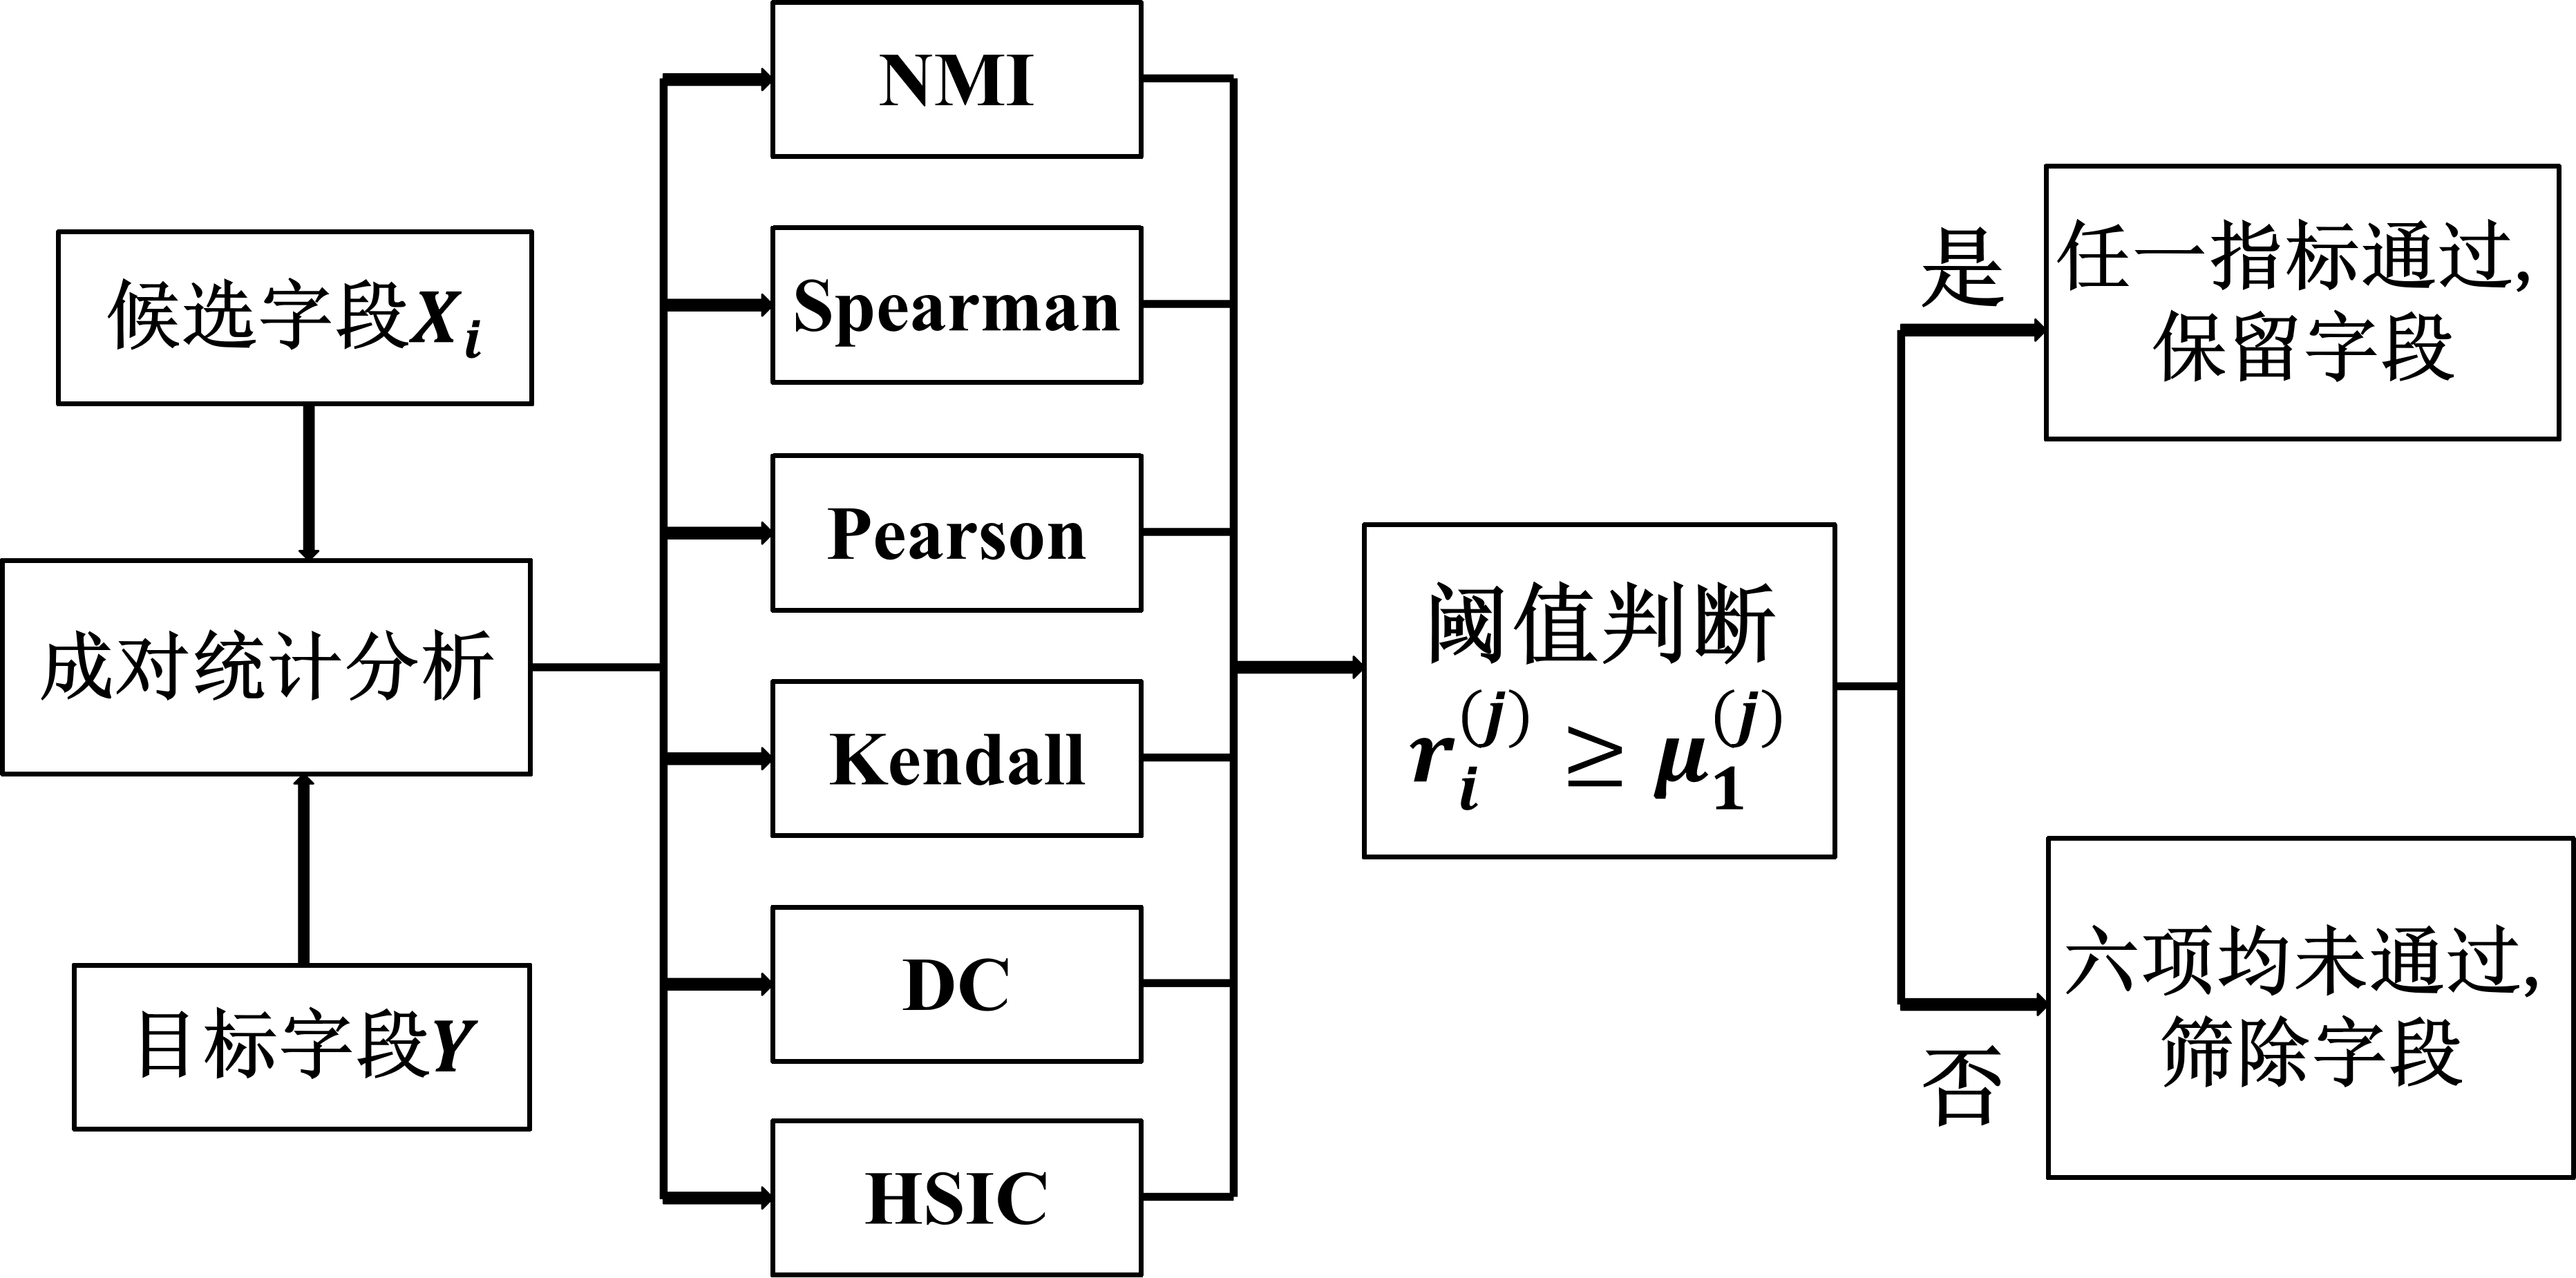
\includegraphics[width=\columnwidth]{初筛流程.png}
\figbicaption{多相关性初筛流程}{Multi-correlation preliminary screening workflow}
\label{fig:screening_flow}
\end{figure}

\subsection{L1 门控深度推断模型}
经过多相关性初筛后，得到候选字段集合 $X=\{X_1,\ldots,X_m\}$，其中 $m$ 为通过初筛的字段数。相关性初筛能够删除明显弱相关字段，但仍会保留大量在统计上有关联、在推断模型中却可能相互替代的字段。若直接使用全部初筛字段训练 DNN，模型虽然可能取得较高 $R^2$，但无法说明哪些输入字段承担主要推断作用。为此，本文在 DNN 输入端引入可学习门控层，其结构如图~\ref{fig:l1_structure} 所示。

\begin{figure}[!htbp]
\centering
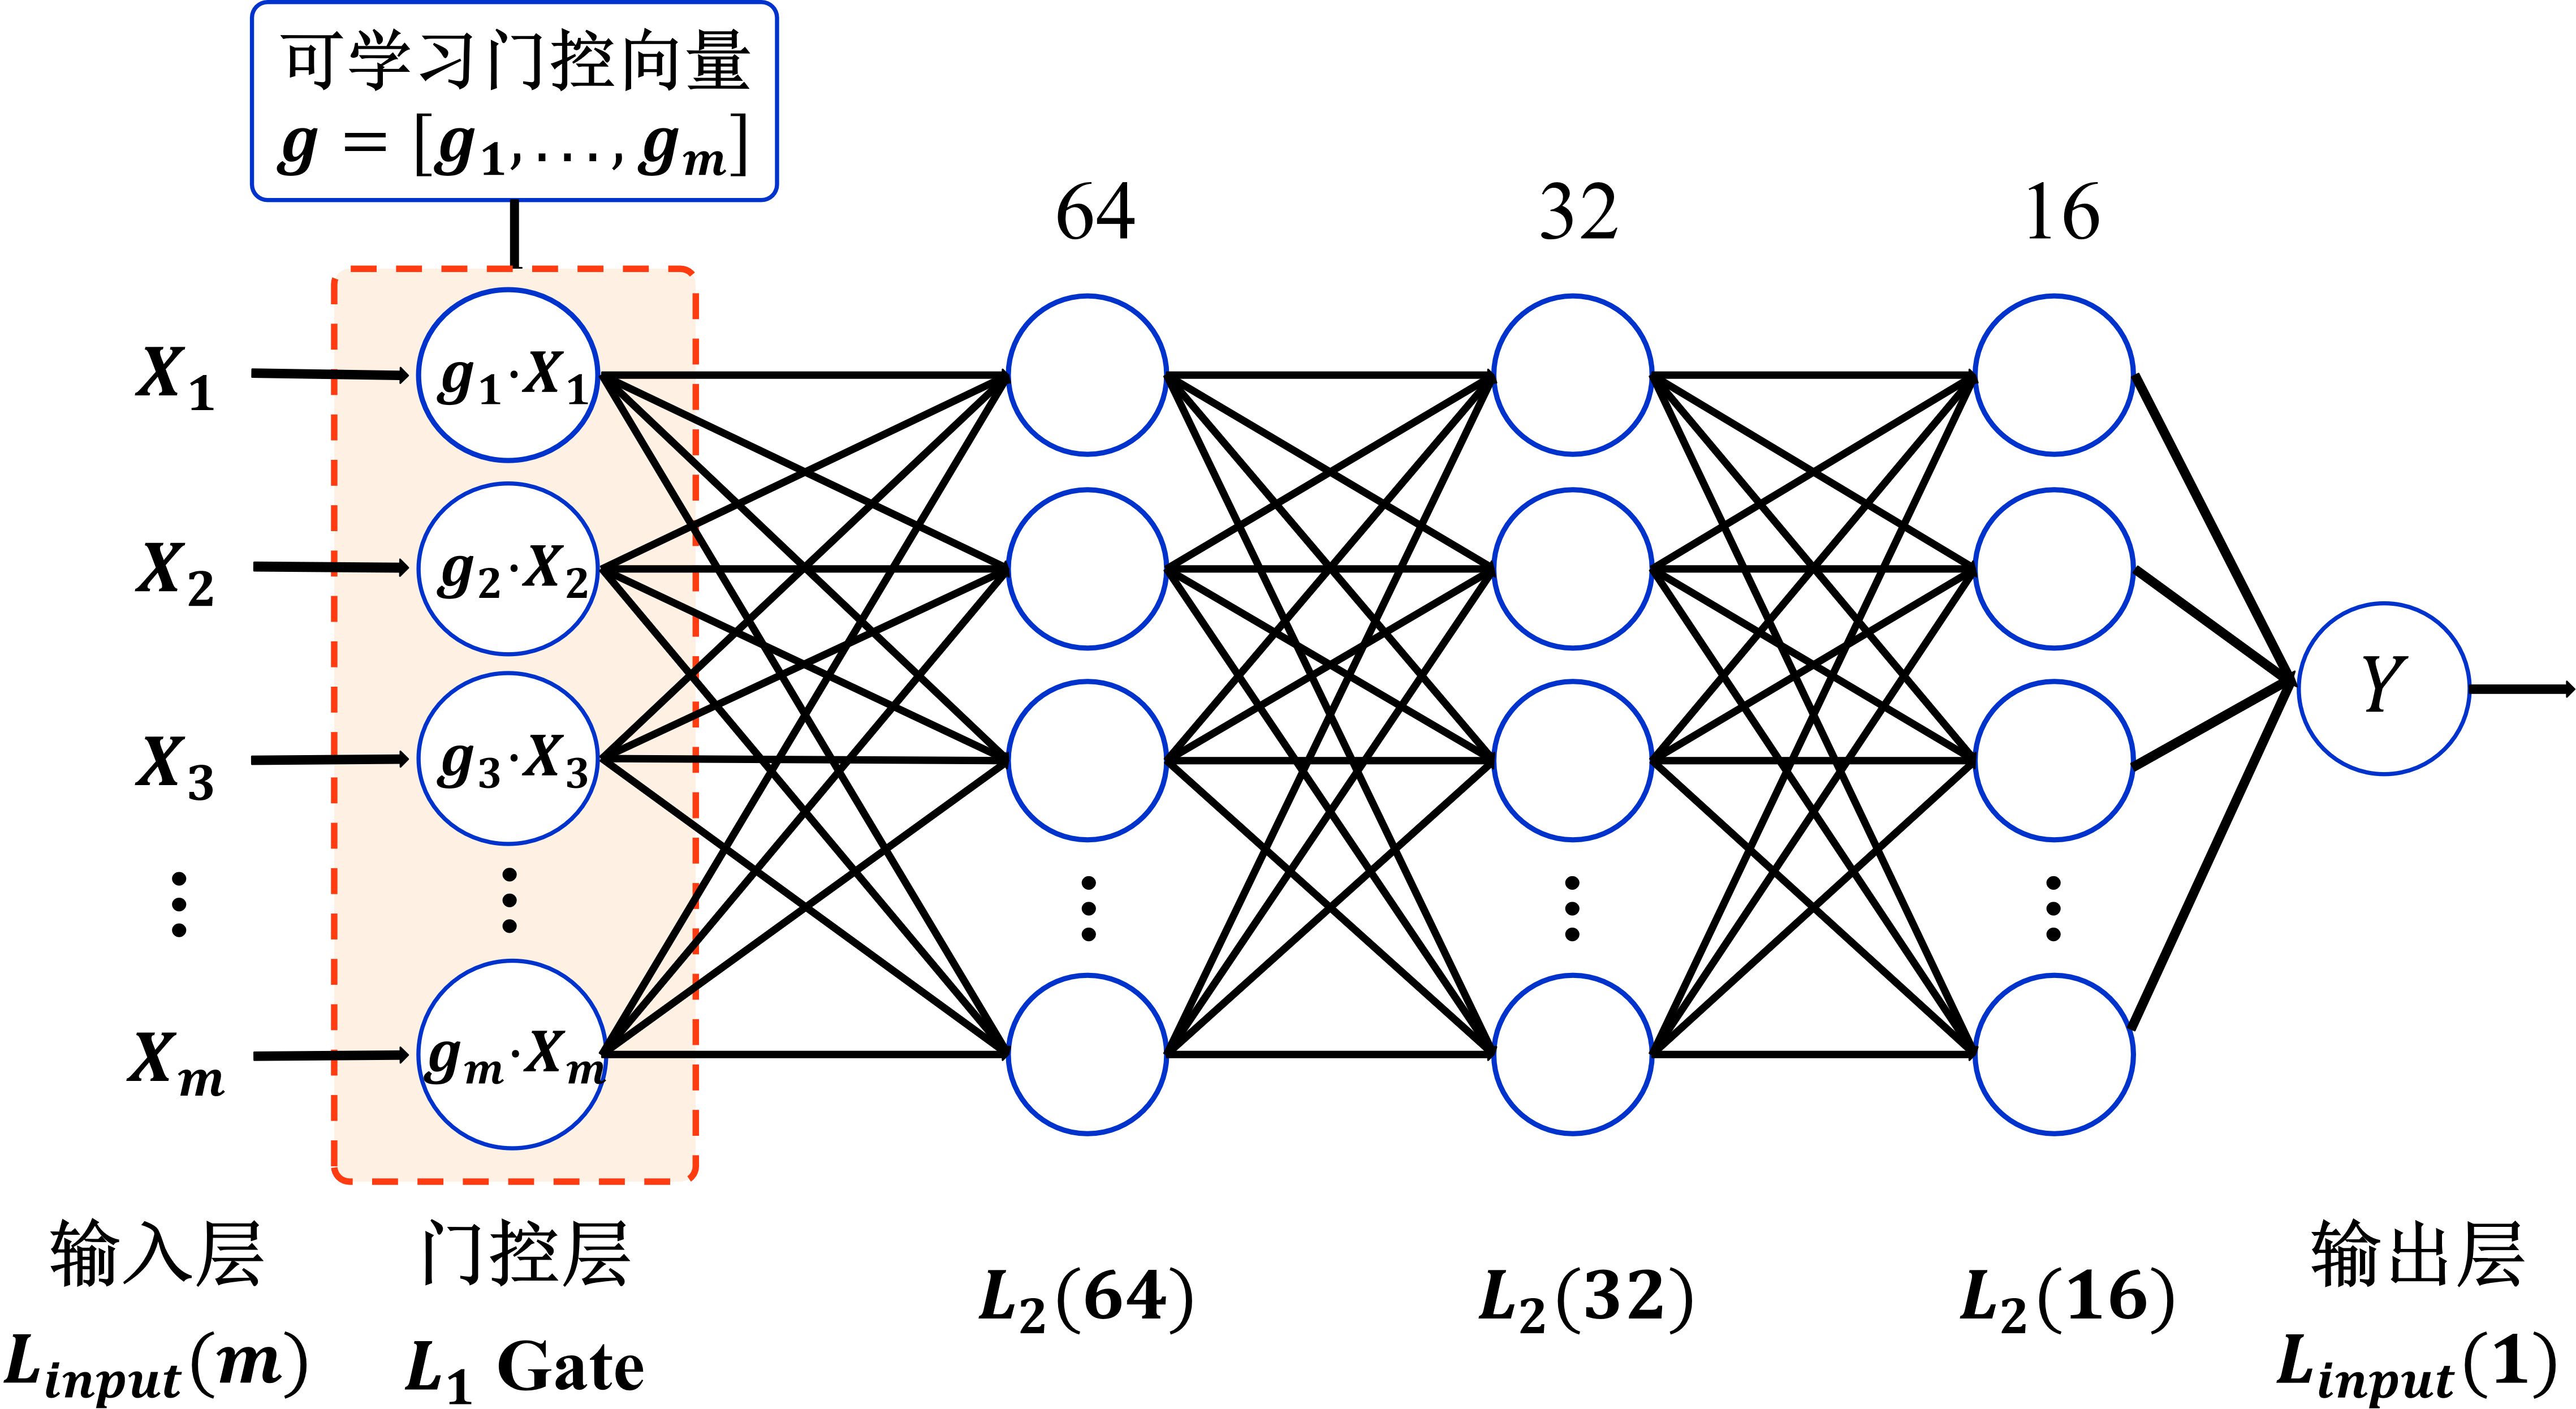
\includegraphics[width=\columnwidth]{门控.png}
\figbicaption{L1 门控深度推断模型结构}{Structure of the L1-gated deep inference model}
\label{fig:l1_structure}
\end{figure}

设门控向量为 $g=[g_1,\ldots,g_m]$，其中 $g_i$ 与候选字段 $X_i$ 一一对应。门控层对输入字段进行逐元素加权，模型输出为
\begin{equation}
\hat{Y}=f_{\theta}(g\odot X),
\end{equation}
式中：$\odot$ 为逐元素相乘运算；$f_{\theta}$ 为由多层全连接网络构成的非线性推断模型。当 $g_i$ 较大时，字段 $X_i$ 的信息能够较充分地进入后续网络；当 $g_i$ 接近 0 时，该字段在前向传播中被显著抑制。为了使门控值既服务于推断精度，又能够产生稀疏选择结果，训练目标函数定义为
\begin{equation}
\mathcal{L}=\frac{1}{n}\sum_{k=1}^{n}(y_k-\hat{y}_k)^2+\lambda\sum_{i=1}^{m}|g_i|.
\end{equation}
式中：第一项为均方误差损失，用于保证模型对目标字段的推断能力；第二项为 L1 正则化惩罚，$\lambda$ 为正则化系数，用于推动门控参数趋向稀疏。该目标函数体现了字段选择中的竞争机制：若某字段能够稳定降低预测误差，反向传播会保留或增大其门控值；若某字段主要提供重复信息、弱相关扰动或噪声，L1 惩罚会持续压低其门控值。与先训练模型再事后解释特征重要性不同，L1 门控将字段筛选嵌入推断模型的训练过程，使字段取舍直接受到目标推断误差的约束。

训练结束后，满足
\begin{equation}
|g_i|\geq \mu_2
\end{equation}
的字段被判定为活跃推断源。式中 $\mu_2$ 为活跃阈值。本文将活跃字段数量记为 $n_s$，并在后续 baseline 对比实验中作为统一字段预算，使不同方法在相同字段数量约束下进行公平比较。为检验门控筛选结果是否独立有效，本文不直接把门控模型的训练结果作为最终结论，而是将选中字段重新输入普通 DNN 进行训练和测试。若再训练模型仍能保持较高 $R^2$，则说明该字段集合确实包含支撑目标字段推断的主要信息。

\subsection{相关性驱动的改进门控}
普通 L1 门控模型能够在推断训练过程中识别活跃字段，但每个门控参数都是独立学习的变量，尚不能直接回答“六类相关性指标分别对最终推断源判定贡献多少”这一问题。前述六类指标虽提供了统计依赖证据，但在普通流程中主要用于初筛，其作用仍停留在描述性分析层面，没有与最终推断导向的门控判定形成统一融合机制。换言之，初筛阈值能够决定某个字段是否进入候选空间，却无法解释不同相关性指标如何共同影响门控的打开或关闭。

这一问题在增量数据分析中尤为突出。假设数据共享方新增一列候选字段，若仍采用普通 L1 门控方法，通常需要把新字段并入候选集合并重新训练推断模型，才能判断其是否构成推断源。若能够学习出不同相关性指标对推断贡献的权重，则可先计算新字段与目标字段之间的六维相关性向量，再通过统一映射快速得到其推断贡献度，从而降低增量字段分析的计算成本。基于这一考虑，本文进一步提出相关性驱动的改进门控模型，其结构如图~\ref{fig:improved_gate_structure} 所示。

\begin{figure}[!htbp]
\centering
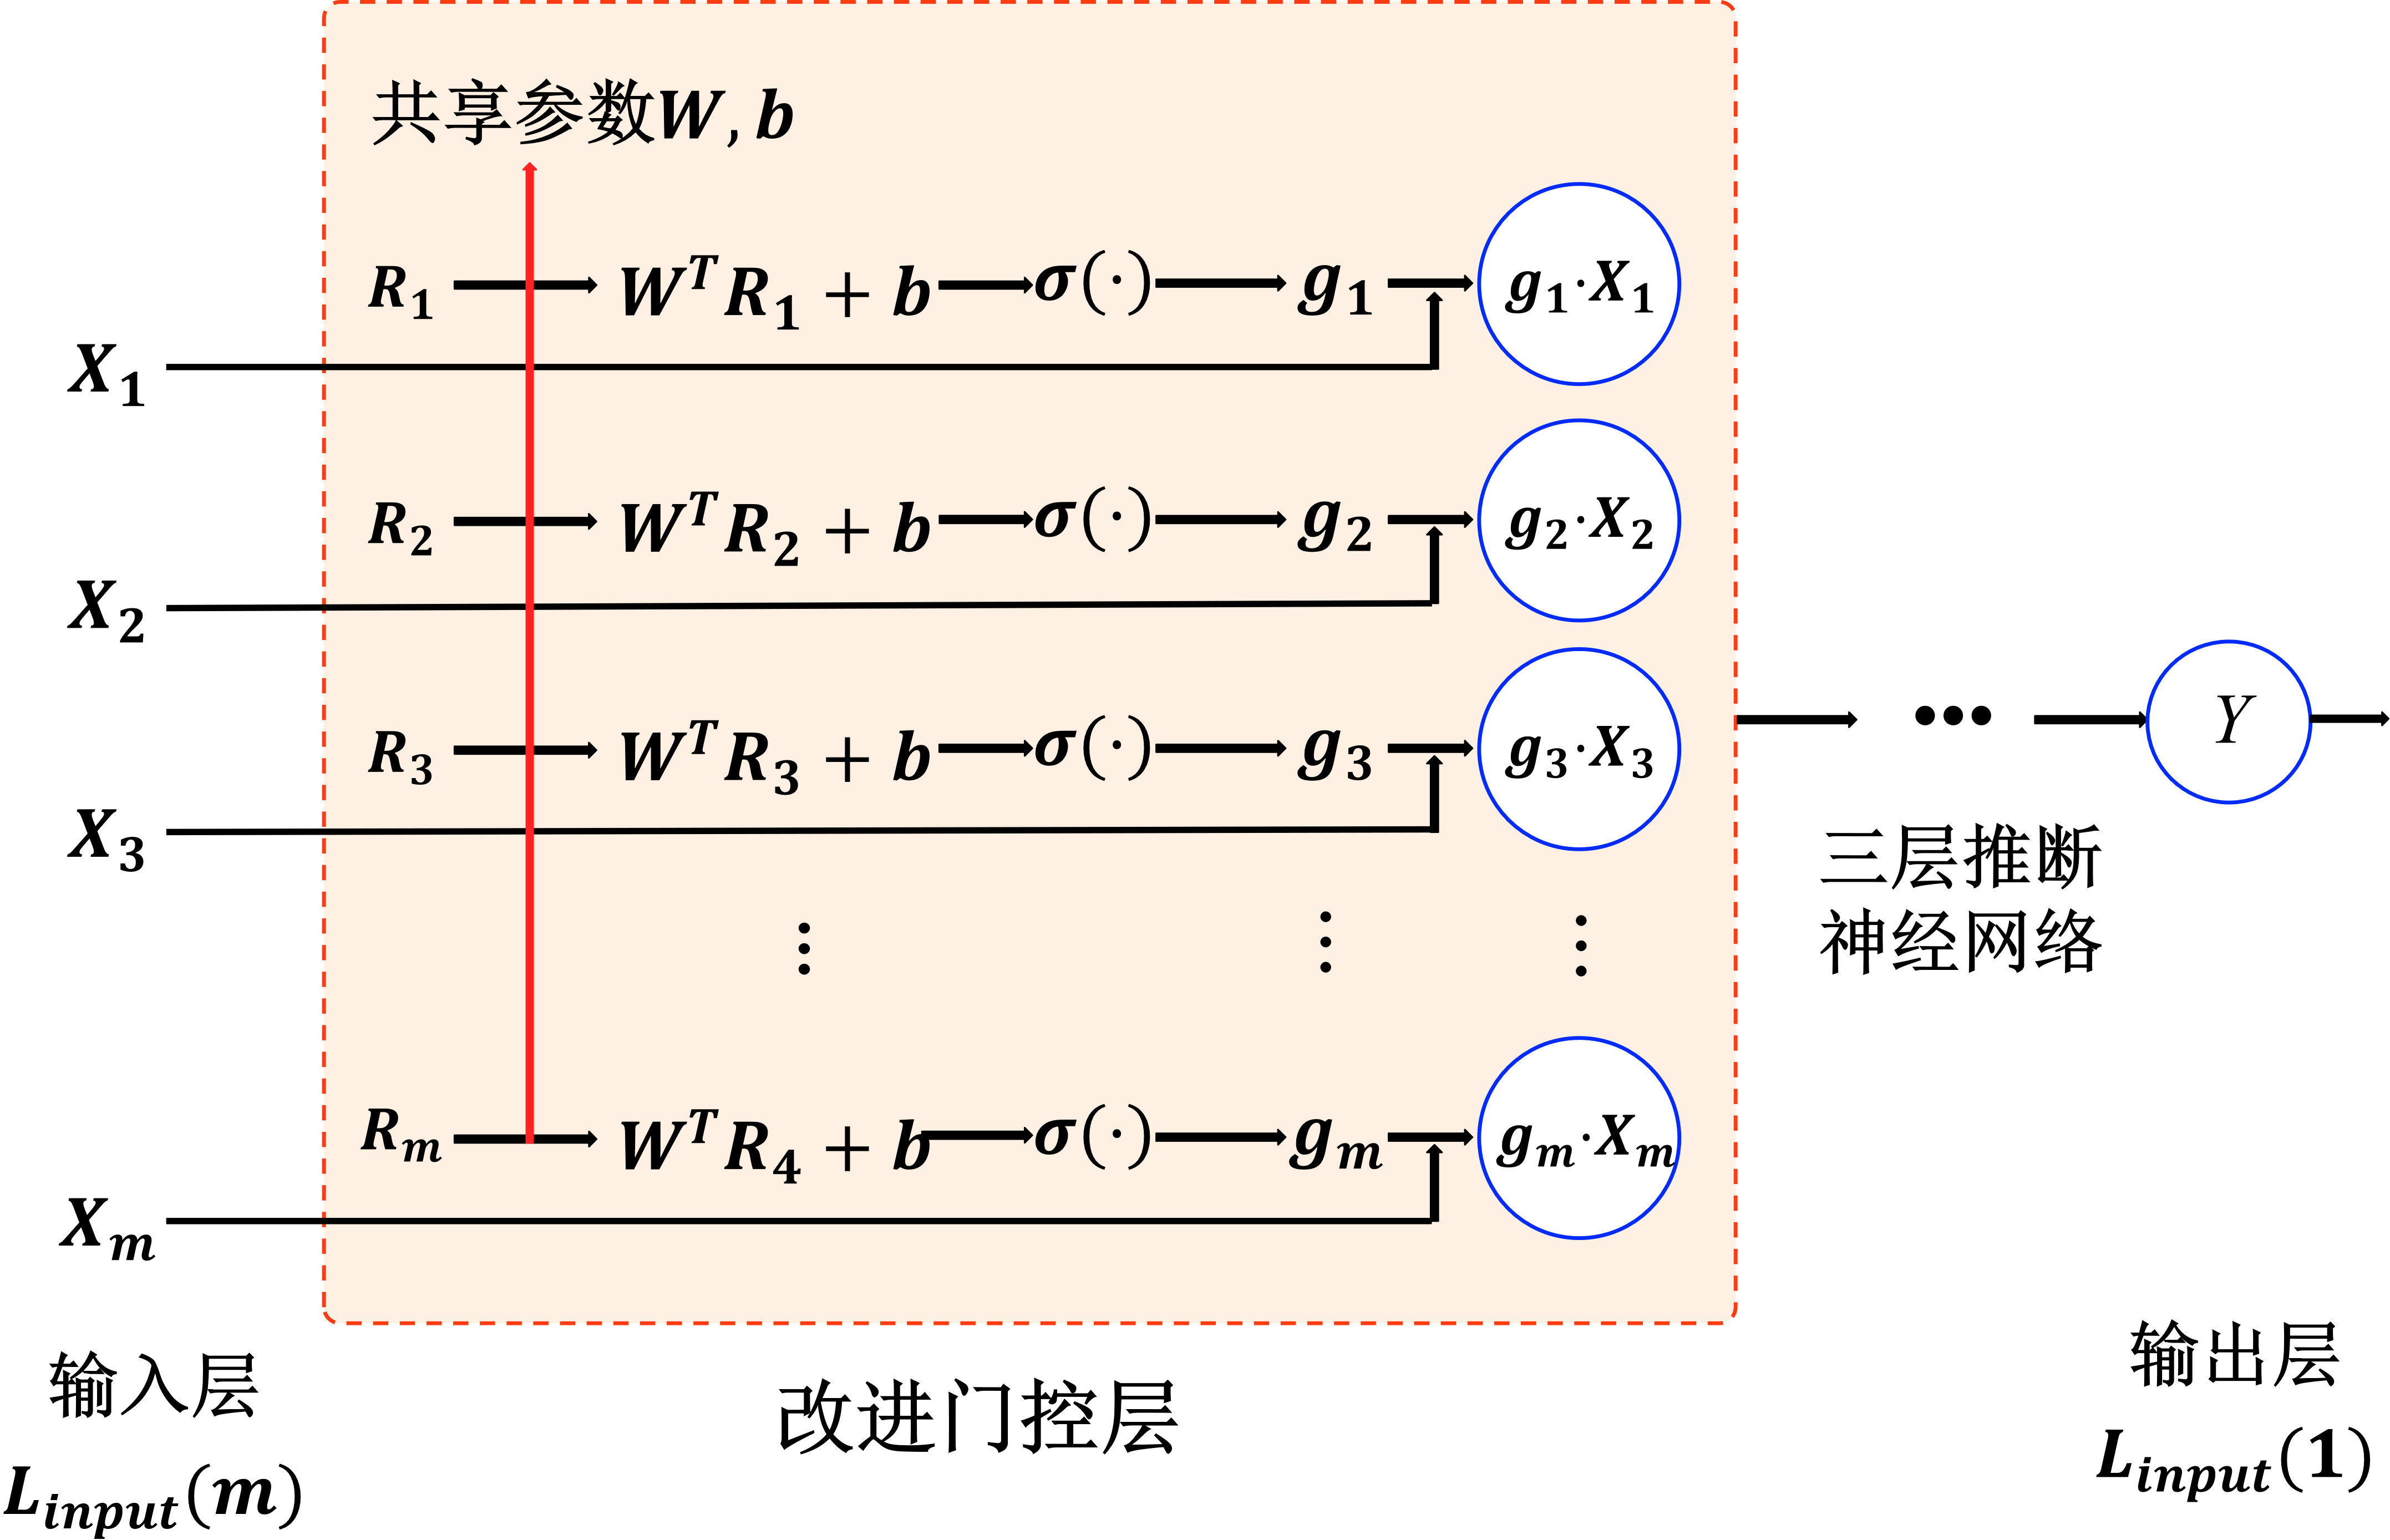
\includegraphics[width=\columnwidth]{改进门控.png}
\figbicaption{相关性驱动的改进门控层结构}{Structure of the correlation-driven improved gate layer}
\label{fig:improved_gate_structure}
\end{figure}

改进门控不再为每个字段直接设置相互独立的自由门控参数，而是将字段 $X_i$ 的六维相关性向量 $R_i$ 作为门控生成依据，通过线性映射和 Sigmoid 激活函数得到门控值：
\begin{equation}
g_i=\sigma(W^{\mathrm{T}}R_i+b),
\end{equation}
式中：$W\in\mathbb{R}^{6}$ 为六类相关性指标对应的可学习权重向量，反映各指标对推断源判定的相对贡献；$b$ 为全局偏置项，可理解为整体的门控开启容忍水平；$\sigma(\cdot)$ 为 Sigmoid 激活函数：
\begin{equation}
\sigma(z)=\frac{1}{1+\mathrm{e}^{-z}}.
\end{equation}
Sigmoid 函数将任意实数映射到 $(0,1)$ 区间，使门控值可解释为字段被打开的连续强度：$z$ 越大，$\sigma(z)$ 越接近 1，字段信息被保留；$z$ 越小则越接近 0，字段信息被抑制。这里选用 Sigmoid 还有一层考虑：其导数 $\sigma'(z)=\sigma(z)[1-\sigma(z)]$ 在 $z=0$ 处取得最大值 0.25，即函数在零点附近变化最为剧烈、对自变量最为灵敏。因此当 $W^{\mathrm{T}}R_i+b$ 落在 0 附近时，门控对相关性证据的细微差异具有最强的分辨能力，可将原本数值接近的字段放大为明显的门控开闭差异，使处于临界状态的字段得到更清晰的区分。相应地，$W^{\mathrm{T}}R_i+b=0$（此时 $g_i=0.5$）自然成为区分推断源与冗余字段的分界：
\begin{equation}
W^{\mathrm{T}}R_i+b=0.
\end{equation}
当 $g_i>0.5$ 时，字段 $X_i$ 的综合相关性证据位于该分界的打开侧，更可能作为推断源进入模型；当 $g_i<0.5$ 时，其证据不足以支持门控打开，更可能为冗余或低贡献字段。训练过程中，$W$、$b$ 与 DNN 主干参数一并优化，并受推断误差与门控稀疏约束的共同影响，因此 $W$ 的取值不仅反映某类相关性指标的统计强弱，更反映其在当前推断任务中的实际有效贡献。

改进门控的价值并不在于单纯追求更高的 $R^2$，而在于：模型在推断与特征稀疏化训练中自动学习到各类相关性指标对推断贡献的相对权重 $W$，并据此学到以六维相关性为输入的字段区分准则 $W^{\mathrm{T}}R_i+b$。这带来两点便利：对已有字段，$W$ 直观给出各指标对门控开闭的贡献；对新增字段，只要已知其与目标的六维相关性，即可由 $g_i=\sigma(W^{\mathrm{T}}R_i+b)$ 直接估计推断贡献度，而无需重训完整模型。相关性分析由此从相互独立的初筛指标，转化为一个数据驱动、可解释的统一推断贡献度量。

\section{实验与结果分析}
\subsection{实验设置}
\subsubsection{数据集}
实验数据采用美国 PJM 互联电网 2025 年小时级市场与运行数据\cite{ref-pjm-dataminer}。选用该数据集主要基于两点考虑：一是 PJM 数据公开可得，便于实验复现与同行验证；二是运行状态数据在电力系统中通常被视为高价值数据，其与大量字段存在复杂关联，正是隐性推断源分析的典型对象。尽管该数据公开发布，但其所反映的潮流约束、市场出清等物理与机制关联，与各类电力系统数据是相通的，因此基于公开数据得到的方法与结论，对真实电力数据的关联分析同样具有参考意义。

该数据集包含 8760 行（对应全年逐小时记录）和 72 列，其中前两列为 UTC 和东部时间的时间戳，仅用于时间对齐，不参与建模分析。去除时间字段后，剩余 70 个数据字段可按照 PJM Data Miner 官方数据源定义划分为如表~\ref{tab:data_overview} 所示的类别。数据涵盖发电与损耗、风电光伏出力、燃料类型发电、负荷预测与计量、调频市场、辅助服务市场、节点电价和交换功率等多个业务领域，字段间存在广泛的物理和市场机制关联。

\begin{table}[!htbp]
\centering
\scriptsize
\setlength{\tabcolsep}{2pt}
\tabbicaption{PJM 2025 数据字段分类概览}{Classification of PJM 2025 data fields}
\label{tab:data_overview}
\begin{tabularx}{\columnwidth}{c>{\raggedright\arraybackslash}p{0.40\columnwidth}X}
\toprule
编号 & Dataset & 中文说明 \\
\midrule
D1--D2 & Generation and EHV Losses & 小时级总发电量与超高压损耗数据。 \\
D3 & Wind Generation & PJM 区域小时级风电出力。 \\
D4 & Solar Generation & PJM 区域小时级光伏出力。 \\
D5--D24 & Generation by Fuel Type & 按燃料类型统计的发电出力与占比。 \\
D25--D26 & Historical Load Forecasts & 日前及最新可用负荷预测。 \\
D27 & Hourly Load: Preliminary & 由遥测数据计算的预估小时负荷。 \\
D28 & Hourly Load: Metered & PJM RTO 服务区域计量负荷。 \\
D29--D37 & Regulation Billing Data & 调频市场预结算相关价格、容量与信用数据。 \\
D38--D56 & Day-Ahead AS Market Results & 日前辅助服务市场的价格、需求与容量结果。 \\
D57--D60 & Day-Ahead Hourly LMPs & 日前能量市场 LMP、拥塞价与边际损耗价。 \\
D61--D64 & Real-Time Hourly LMPs & 实时能量市场 LMP、拥塞价与边际损耗价。 \\
D65--D70 & Actual/Schedule Summary & 净/总实际、计划和非计划交换功率。 \\
\bottomrule
\end{tabularx}
\end{table}

\subsubsection{参数设置}
多相关性初筛阶段的各项阈值设置如下：NMI 为 0.06、Spearman 秩相关系数为 0.15、Pearson 相关系数为 0.15、Kendall 秩相关系数为 0.12、距离相关系数为 0.20、HSIC 为 0.25，均用于“任一指标通过即保留”的宽松初筛规则。DNN 主干采用三层全连接隐藏层，各层神经元数量依次为 64、32 和 16；优化器采用 Adam\cite{ref-kingma-adam}；批次大小为 50；训练轮数为 200；随机种子固定为 42 以保证可重复性。普通 L1 门控模型的 L1 正则化系数 $\lambda$ 设为 0.002，活跃阈值 $\mu_2$ 设为 0.10。改进 L1 门控模型的门控判定阈值为 0.50，L1 正则化系数设为 0.016，权重向量 $W$ 和偏置 $b$ 分别配置独立学习率，以确保相关性权重和门控偏置的稳定收敛。

\subsubsection{实验设计}
围绕所提方法，本文从单目标分析、多目标对比与机理解释三个层面设计实验，分别对应后续三节。第 3.2 节为单目标推断源识别与门控演化分析，以一个核心运行量为目标，展示多相关性初筛、门控收缩、Top-n 验证与改进门控的完整过程；第 3.3 节为多目标对比实验，在 12 个目标字段上将 L1 门控与全量 DNN 直接对比，并在统一字段预算下与多种特征选择方法进行同预算比较；第 3.4 节为冗余信息影响分析，通过训练曲线与 Top-n 递增实验，解释少量字段推断精度反优于全量字段的内在原因。

为保证比较公平，全文统一约定：全量 DNN 使用扣除目标后的全部 69 个数值字段作为输入；L1DNN 则先由 L1 门控确定推断源集合，再以相同 DNN 结构重新训练与评估；同预算比较中各方法在相同字段数下选取字段并统一以普通 DNN 训练和测试，从而使比较聚焦于字段选择质量而非字段数量差异。

\subsection{单目标推断源识别与门控演化}
本节以单一核心运行量为目标，完整呈现所提方法的工作过程：多相关性初筛、推断精度与门控收缩、Top-n 验证以及改进门控学习。

\subsubsection{多相关性初筛结果}
净实际交换功率（\code{net\_actual\_interchange\_mw}）反映区域间的实时电力交换，是电网运行的核心状态量之一，通常具有较高的分析价值，且与发电、负荷、电价和辅助服务等众多字段存在复杂关联，适合作为隐性推断源分析的中心目标。以其为目标，对扣除该字段后的 69 个候选关系进行六类指标综合评估，最终保留 55 个候选字段，筛除 14 个与目标整体相关性微弱的字段。六类指标各自通过的字段数在 23～33 之间；按通过的指标数统计，14 个字段未通过任何指标而被筛除，4 个字段通过全部六项，其余字段通过 1～5 项不等。

表~\ref{tab:screening_top} 按最大绝对相关得分给出初筛结果节选。可见辅助服务、交换功率与燃料结构等字段在多类指标下均呈现较强依赖，说明净实际交换功率的潜在推断路径涉及多个业务领域，而非由单一线性关系决定。

\begin{table}[!htbp]
\centering
\scriptsize
\setlength{\tabcolsep}{1pt}
\tabbicaption{净实际交换功率目标的多相关性初筛结果节选}{Partial multi-correlation screening results for net actual interchange}
\label{tab:screening_top}
\begin{tabularx}{\columnwidth}{cXrrrrrrc}
\toprule
排名 & 字段 & NMI & Spear. & Pear. & Kend. & DC & HSIC & 通过数 \\
\midrule
1 & 30 min备用实际量 & 0.076 & -0.430 & -0.394 & -0.289 & 0.403 & 0.856 & 6 \\
2 & 30 min备用总量 & 0.067 & -0.428 & -0.397 & -0.252 & 0.374 & 0.845 & 6 \\
3 & 总计划交换功率 & 0.133 & -0.465 & -0.483 & -0.318 & 0.458 & 0.813 & 6 \\
4 & 核电出力 & 0.116 & -0.354 & -0.424 & -0.248 & 0.442 & 0.795 & 6 \\
\multicolumn{9}{c}{\(\cdots\)} \\
53 & 实时拥塞价 & 0.013 & 0.124 & 0.155 & 0.091 & 0.182 & 0.032 & 1 \\
54 & 同步备用MCP & 0.050 & 0.175 & 0.133 & 0.111 & 0.134 & 0.063 & 1 \\
55 & 日前拥塞价 & 0.073 & -0.039 & -0.066 & -0.048 & 0.171 & 0.070 & 1 \\
\bottomrule
\end{tabularx}
\end{table}

\subsubsection{推断精度与门控收缩过程}
图~\ref{fig:train_pair} 对比了两个模型的训练过程：全量 DNN（69 字段）最优测试 $R^2$ 为 0.9675，L1 门控模型为 0.9775。可见稀疏门控不仅未削弱推断能力，反而提升了泛化性能——因其持续压缩冗余字段贡献，迫使模型集中利用稳定推断路径，从而降低过拟合倾向。

\begin{figure}[!htbp]
\centering
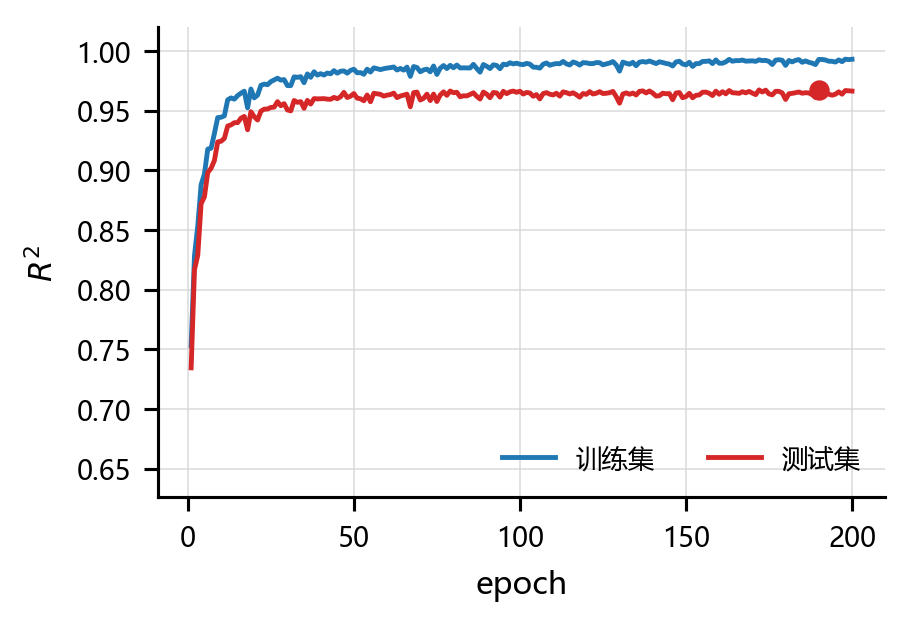
\includegraphics[width=\columnwidth]{net_train_dnn_r2_zh.png}\\[-0.2em]
{\scriptsize (a) 全量 DNN}\\[0.45em]
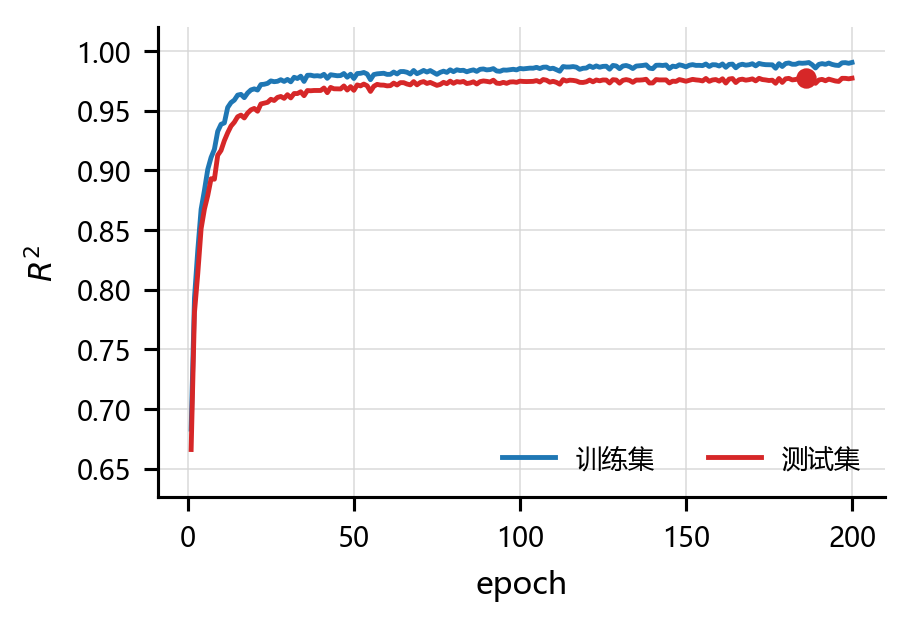
\includegraphics[width=\columnwidth]{net_train_l1_r2_zh.png}\\[-0.2em]
{\scriptsize (b) L1 门控模型}
\figbicaption{净实际交换功率目标上的 $R^2$ 训练过程对比}{Comparison of training $R^2$ processes for net actual interchange}
\label{fig:train_pair}
\end{figure}

图~\ref{fig:l1_gate} 展示了门控参数的演化轨迹：训练初期各字段门控值即分化，随着 L1 惩罚的持续作用，大量弱贡献字段衰减至阈值以下，仅少数关键字段维持较高门控值，在 $\mu_2=0.10$ 下最终保留 18 个活跃字段（含天然气与煤电出力、实时负荷、光伏出力等运行变量）。图~\ref{fig:l1_active} 显示活跃字段数随训练逐步下降并趋于稳定，说明 L1 门控并非一次性截断弱字段，而是在优化中借助梯度信息逐步剔除冗余，最终形成紧凑的推断源集合。

\begin{figure}[!htbp]
\centering

\includegraphics[width=\columnwidth]{net_l1_gate_params_zh.png}
\figbicaption{净实际交换功率目标上门控参数的演化过程}{Evolution of gate parameters for net actual interchange}
\label{fig:l1_gate}
\end{figure}

\begin{figure}[!htbp]
\centering

\includegraphics[width=\columnwidth]{net_l1_active_features_zh.png}
\figbicaption{净实际交换功率目标上活跃字段数量的变化}{Number of active features over training epochs}
\label{fig:l1_active}
\end{figure}

\subsubsection{Top-n 推断源验证}
为验证所选字段的实际推断能力，按门控值依次取 Top3 至 Top18 字段分别训练 DNN 评估测试 $R^2$，并与全量 69 字段及其余未选中字段比较，结果如图~\ref{fig:top_series} 所示。

字段过少时推断能力受限（Top3、Top6 仅 0.4469、0.5778），随字段增加迅速提升，Top9 即达 0.9186，Top18 达 0.9681，略高于全量 69 字段的 0.9661；而去除这 18 个推断源后，其余 51 个字段单独训练仅得 0.7820。这表明所选字段共同构成支撑目标推断的核心路径，其余字段虽多却缺乏关键路径。可见 L1 门控识别的是能联合支撑推断的非冗余组合，而非个别强相关字段。

\begin{figure}[!htbp]
\centering

\includegraphics[width=\columnwidth]{net_top_series_r2_zh.png}
\figbicaption{净实际交换功率目标上的 Top-n 推断源验证结果}{Top-n inference-source validation for net actual interchange}
\label{fig:top_series}
\end{figure}

\subsubsection{改进门控的判定边界学习}
图~\ref{fig:improved_gate} 至图~\ref{fig:improved_b} 展示了相关性驱动改进门控模型的训练结果。与普通 L1 门控为每个字段独立学习门控参数不同，改进门控的门控值由六维相关性向量经 Sigmoid 映射生成，其开闭取决于各类相关性指标的加权组合 $W^{\mathrm{T}}R_i+b$：该值越大，门控越倾向打开、字段越可能作为推断源；越小则越倾向关闭，对应冗余或低贡献字段。

改进门控最终保留 17 个活跃字段，最优测试 $R^2$ 为 0.9726。从权重向量 $W$ 的演化看，HSIC 对应权重在收敛后保持最高，表明非线性依赖证据对净实际交换功率的推断贡献最为显著；偏置 $b$ 由接近零逐步降至约 $-0.70$，反映模型在 L1 正则化压力下不断收紧门控打开条件。可见各指标的贡献权重及其组合方式均由数据自动学得，无需人工设定阈值，从而以统一、可解释的方式刻画了各相关性指标对推断源判定的相对贡献。

\begin{figure}[!htbp]
\centering

\includegraphics[width=\columnwidth]{improved_l1_gate_params_zh.png}
\figbicaption{改进 L1 门控模型的门控值演化}{Gate value evolution of the improved L1-gated model}
\label{fig:improved_gate}
\end{figure}

\begin{figure}[!htbp]
\centering
\begin{minipage}{\columnwidth}
\centering
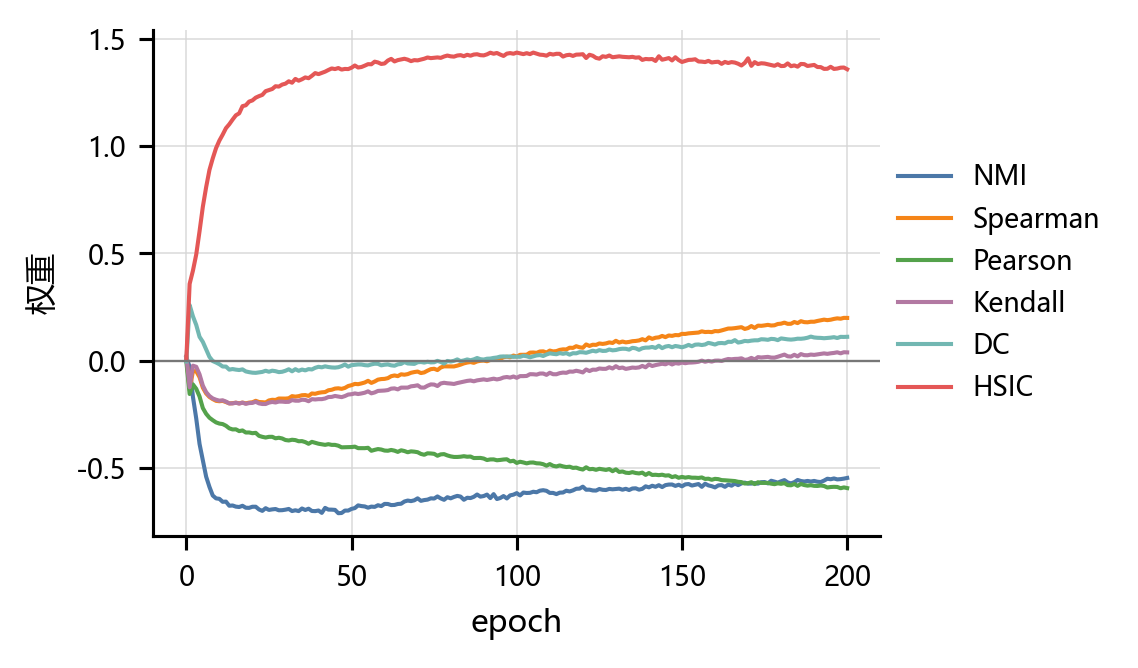
\includegraphics[width=0.92\linewidth]{improved_l1_w_meta_zh.png}\\[-0.4em]
{\scriptsize (a) 相关性指标权重 $W$ 的演化}
\end{minipage}\\[-0.2em]
\begin{minipage}{\columnwidth}
\centering

\includegraphics[width=0.86\linewidth]{improved_l1_b_meta_zh.png}\\[-0.4em]
{\scriptsize (b) 偏置 $b$ 的演化}
\end{minipage}
\figbicaption{改进门控中指标权重与偏置的训练演化}{Evolution of metric weights and bias in the improved gate}
\label{fig:improved_b}
\end{figure}

\subsection{多目标对比实验}
为检验所提方法在不同目标上的普适性，本节在 12 个目标字段上开展两组对比：先将 L1 门控与全量 DNN 直接对比，考察字段大幅压缩后推断能力的保持情况；再在统一字段预算下，将 L1 门控与多种主流特征选择方法进行同预算比较，以排除字段数量差异的干扰。

\subsubsection{全量模型与 L1 门控模型对比}
本组对比中，全量 DNN 以全部 69 个字段为输入训练，L1DNN 则先由 L1 门控确定推断源集合，再以相同网络结构重新训练并评估，结果如图~\ref{fig:dnn_l1_compare} 和表~\ref{tab:dnn_l1_compare} 所示。

以扣除目标后的 69 个字段为统一全量基准（利用率 100\%），12 个目标的全量 DNN 平均测试 $R^2$ 为 0.9031；L1 门控平均仅用 15.50 个字段（利用率约 22.46\%）即取得 0.9111 的平均 $R^2$，整体优于全量 DNN。分目标看，在日前拥塞价、主备用容量、总实际交换与净实际交换等目标上 L1 门控明显或略优，仅在实时拥塞价与日前 LMP 上略低且降幅有限。可见所提方法并非机械式压缩字段，而能在多数目标上以大幅缩减的字段规模保持同等甚至更优的泛化能力。

\begin{figure}[!htbp]
\centering

\includegraphics[width=\columnwidth]{dnn_vs_l1_method_compare_zh.png}
\figbicaption{12 个目标字段上全量 DNN 与 L1 门控模型的测试 $R^2$ 对比}{Comparison of test $R^2$ between all-feature DNN and L1-gated model across 12 targets}
\label{fig:dnn_l1_compare}
\end{figure}

\begin{table}[!htbp]
\centering
\scriptsize
\setlength{\tabcolsep}{2pt}
\tabbicaption{全量 DNN 与 L1 门控选中特征 DNN 的详细对比}{Detailed comparison between all-feature DNN and L1-gated selected-feature DNN}
\label{tab:dnn_l1_compare}
\begin{tabularx}{\columnwidth}{Xrrrr}
\toprule
中心目标 & 全量字段 & L1 字段 & 全量 DNN & L1DNN \\
\midrule
拥塞价 DA & 69 & 2 & 0.9408 & \textbf{0.9954} \\
主备用容量 & 69 & 14 & 0.8495 & \textbf{0.8826} \\
总实际交换 & 69 & 16 & 0.8499 & \textbf{0.8677} \\
30 min 备用容量 & 69 & 22 & 0.8967 & \textbf{0.9086} \\
边际损耗价 DA & 69 & 18 & 0.8936 & 0.8995 \\
净实际交换 & 69 & 18 & 0.9680 & 0.9728 \\
总发电量 & 69 & 16 & 0.9253 & 0.9271 \\
净计划交换 & 69 & 16 & 0.9691 & 0.9694 \\
总损耗 & 69 & 18 & 0.9413 & 0.9409 \\
计量负荷 & 69 & 15 & 0.9157 & 0.9139 \\
日前 LMP & 69 & 13 & \textbf{0.9622} & 0.9510 \\
拥塞价 RT & 69 & 18 & \textbf{0.7255} & 0.7040 \\
\midrule
平均 & -- & 15.5 & 0.9031 & 0.9111 \\
\bottomrule
\end{tabularx}
\end{table}

\subsubsection{同预算基准方法对比}
为避免比较结果受字段数量差异的影响，本文采用统一预算策略进行对比。具体做法为：首先利用 L1 门控在特征预算序列上搜索，确定使其 $R^2$ 达到全量 DNN 的 95\% 或 97\% 水平时对应的字段数 $n$；若遍历候选预算后仍无法达到目标水平，则取当前可获得的最优预算。随后，所有基准方法在相同字段数 $n$ 下进行字段选择，并统一使用普通 DNN 训练和测试。如此，比较即聚焦于“相同字段预算下何种方法所选字段更具推断能力”，而非字段数量多寡。

各目标与平均结果分别如图~\ref{fig:budget_lines} 和图~\ref{fig:budget_avg} 所示。95\% 预算（平均 8.92 个字段）下，L1 门控平均 $R^2$ 为 0.8875，明显高于随机森林（0.8562）、ElasticNet（0.8115）、Lasso（0.7967）与 XGBoost（0.7798）；97\% 预算（平均 9.75 个字段）下其 $R^2$ 进一步升至 0.8943，仍居首位。单相关性排序方法整体偏低，说明仅靠单一指标难以稳定保留联合推断所需的关键字段；树模型与线性稀疏模型虽在个别目标上有竞争力，平均性能仍不及 L1 门控。这验证了所提方法在统一预算约束下的特征选择优势。

\begin{figure}[!htbp]
\centering
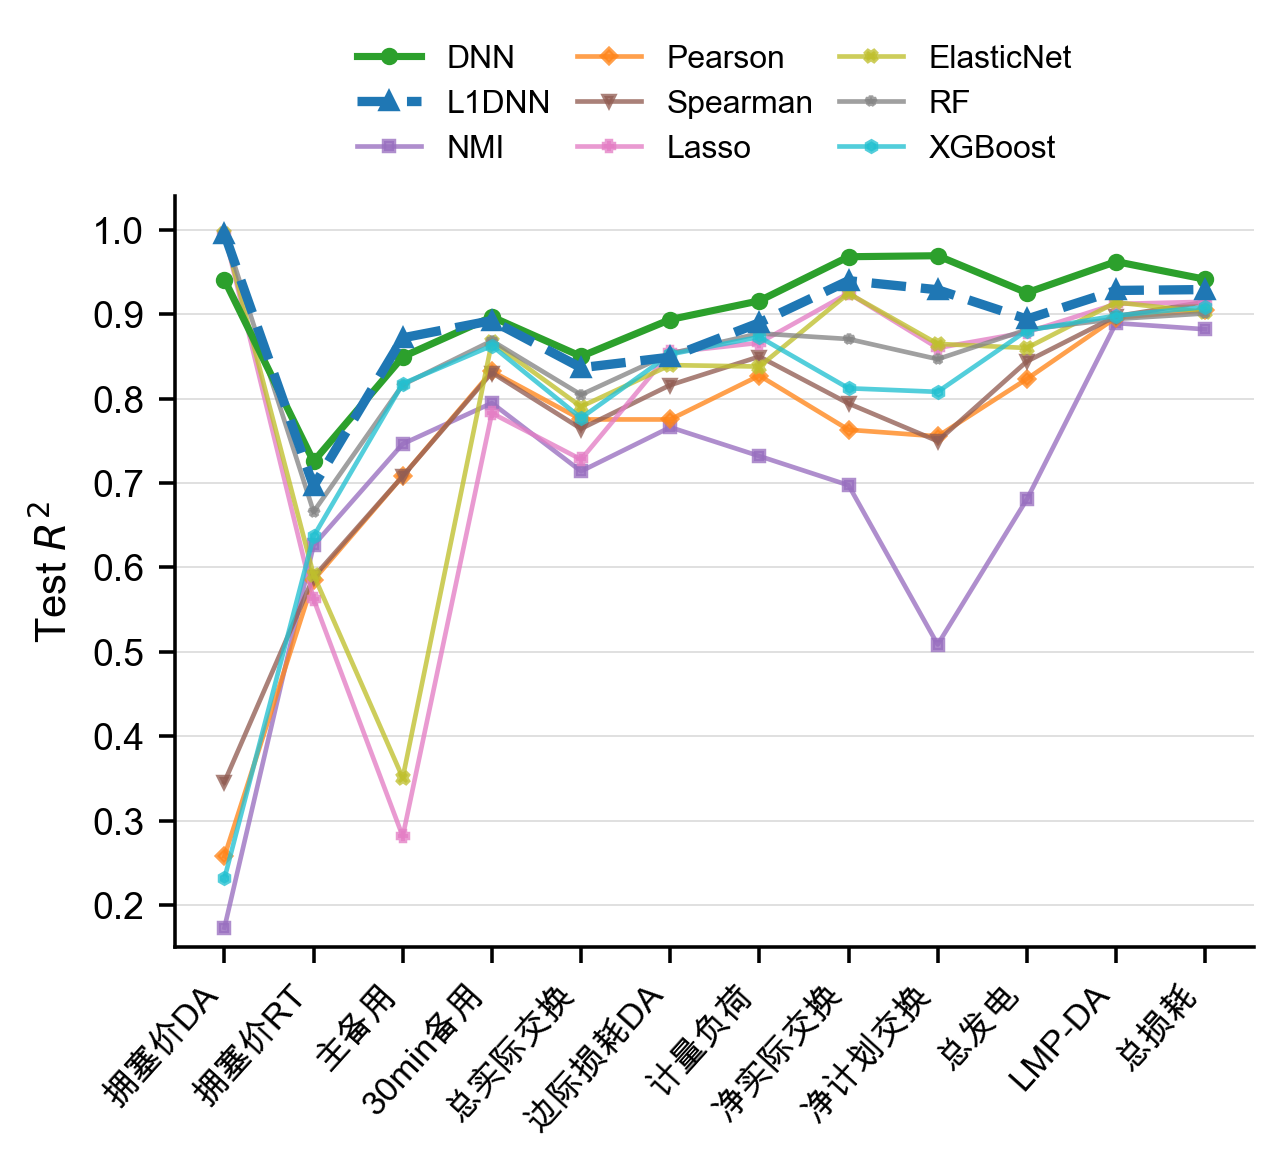
\includegraphics[width=\columnwidth]{budget95_baseline_lines_zh.png}\\[-0.2em]
{\scriptsize (a) 95\% 统一预算}\\[0.45em]
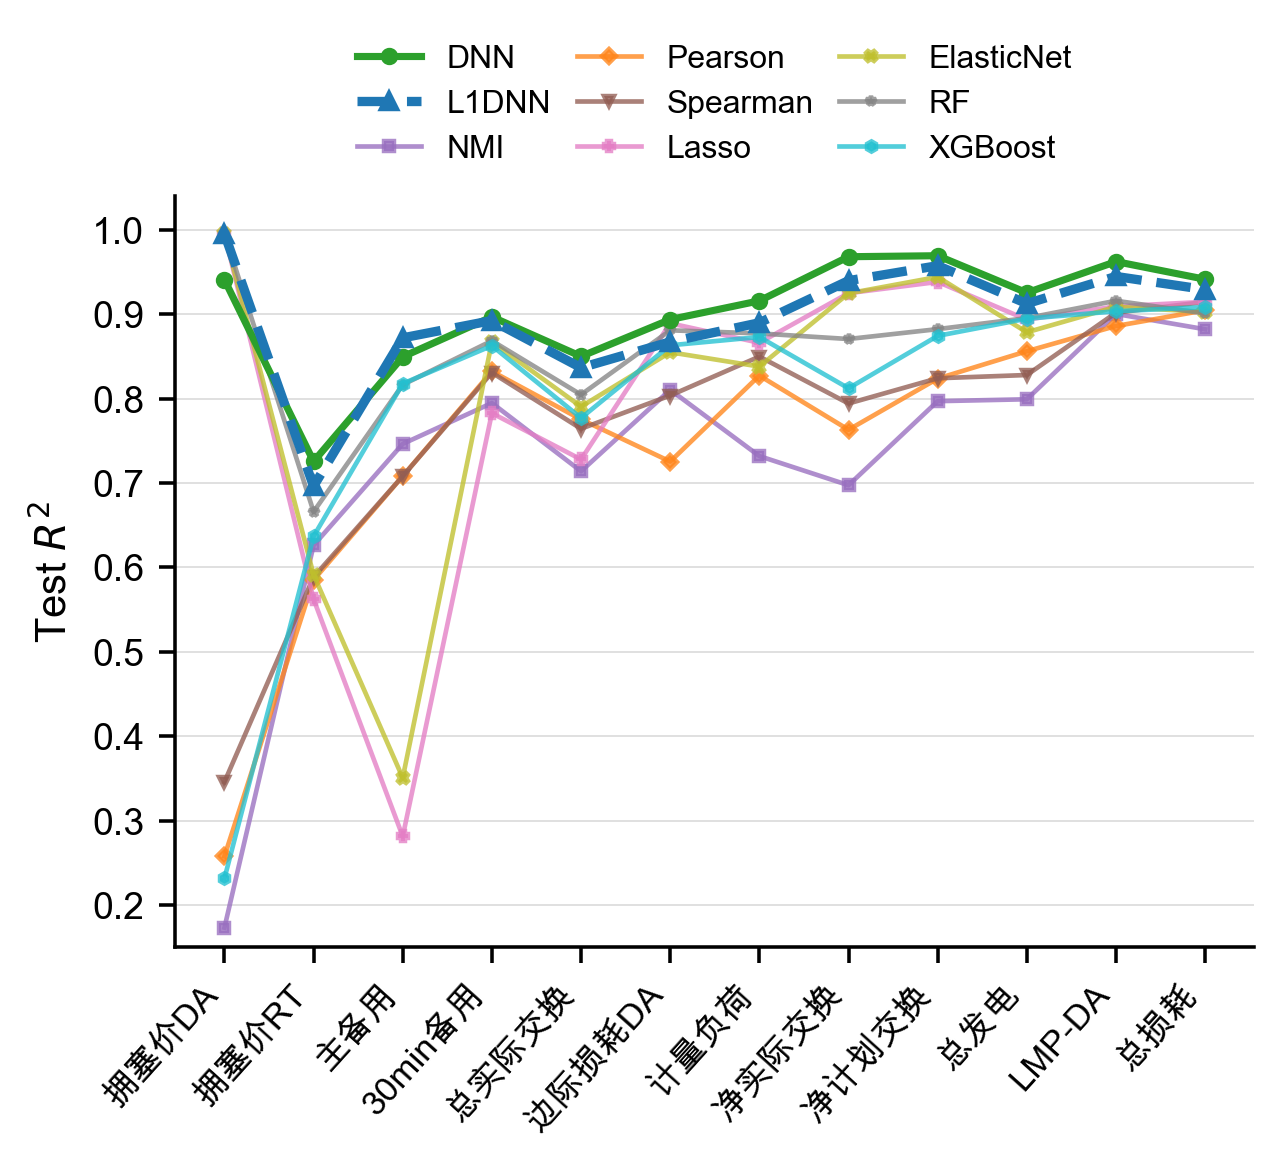
\includegraphics[width=\columnwidth]{budget97_baseline_lines_zh.png}\\[-0.2em]
{\scriptsize (b) 97\% 统一预算}
\figbicaption{统一预算下各目标的基准方法测试 $R^2$ 对比}{Target-level baseline comparison under unified feature budgets}
\label{fig:budget_lines}
\end{figure}

\begin{figure}[!htbp]
\centering
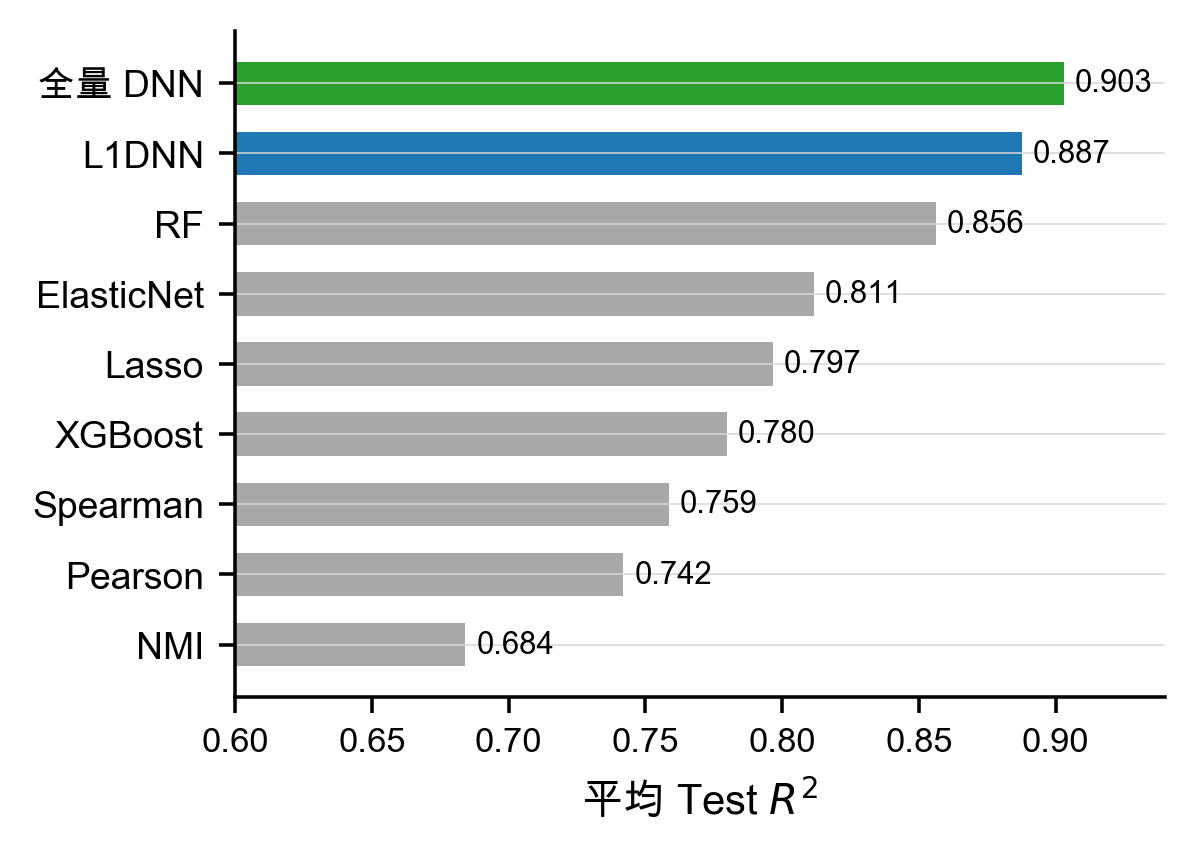
\includegraphics[width=\columnwidth]{budget95_average_bar_zh.png}\\[-0.2em]
{\scriptsize (a) 95\% 统一预算}\\[0.45em]
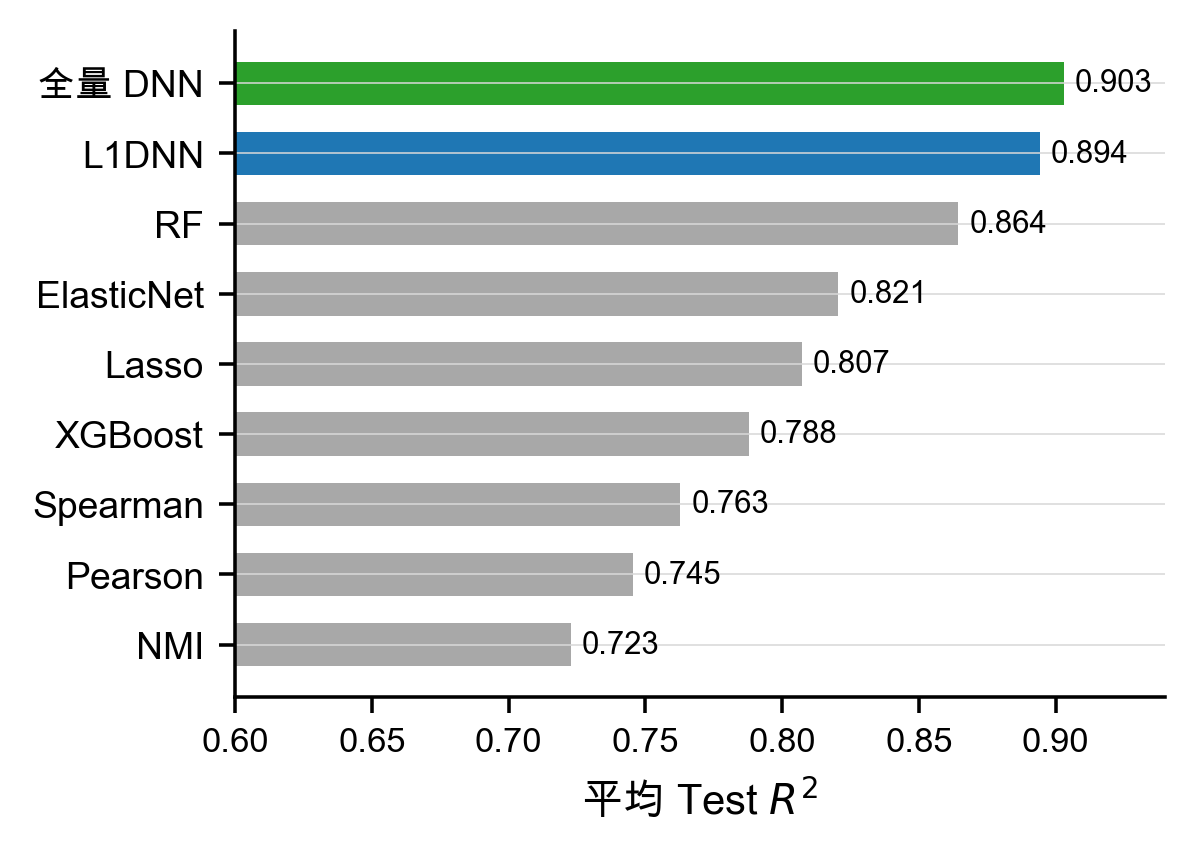
\includegraphics[width=\columnwidth]{budget97_average_bar_zh.png}\\[-0.2em]
{\scriptsize (b) 97\% 统一预算}
\figbicaption{统一预算下各基准方法的平均测试 $R^2$}{Average test $R^2$ of baseline methods under unified feature budgets}
\label{fig:budget_avg}
\end{figure}

\subsection{冗余信息影响分析}
前述实验中，多个目标出现了字段更少的 L1 门控模型推断精度反优于全量模型的现象。为解释其机理，本节从两方面分析：对比全量与压缩字段集的训练曲线以考察泛化差距，并按门控排名逐步增加输入字段以观察精度随字段数的变化。

\subsubsection{训练曲线对比分析}
这一看似反直觉的现象并非因全量字段信息不足，而是源于冗余和噪声字段对深度模型泛化的负面影响：高维输入下，多层感知器在有限样本中易对弱相关字段过拟合，表现为训练拟合持续提升而测试性能下降；Dropout 等正则化手段\cite{ref-he-dropout}虽可缓解过拟合，却难以显式剔除无关字段。为验证上述分析，选取性能差异较显著的日前拥塞价与主备用容量两个目标，对比全量 DNN、L1 门控与 L1 选中特征再训练 DNN 的训练曲线，结果如图~\ref{fig:redundant_curve} 和表~\ref{tab:noise_curve} 所示。

以日前拥塞价为例，全量 DNN（69 字段）测试 $R^2$ 为 0.9408、泛化差距约 0.0621，而仅用 L1 选出的 2 个字段再训练即达 0.9954、泛化差距骤降至 0.0025；主备用容量目标上，全量 DNN 泛化差距约 0.1439，L1 选中特征（35 字段）将测试 $R^2$ 由 0.8495 提升至 0.8580 并改善了泛化差距。可见字段压缩降低了模型对弱相关与噪声字段的过度记忆，使测试表现更稳定。

\begin{figure}[!htbp]
\centering
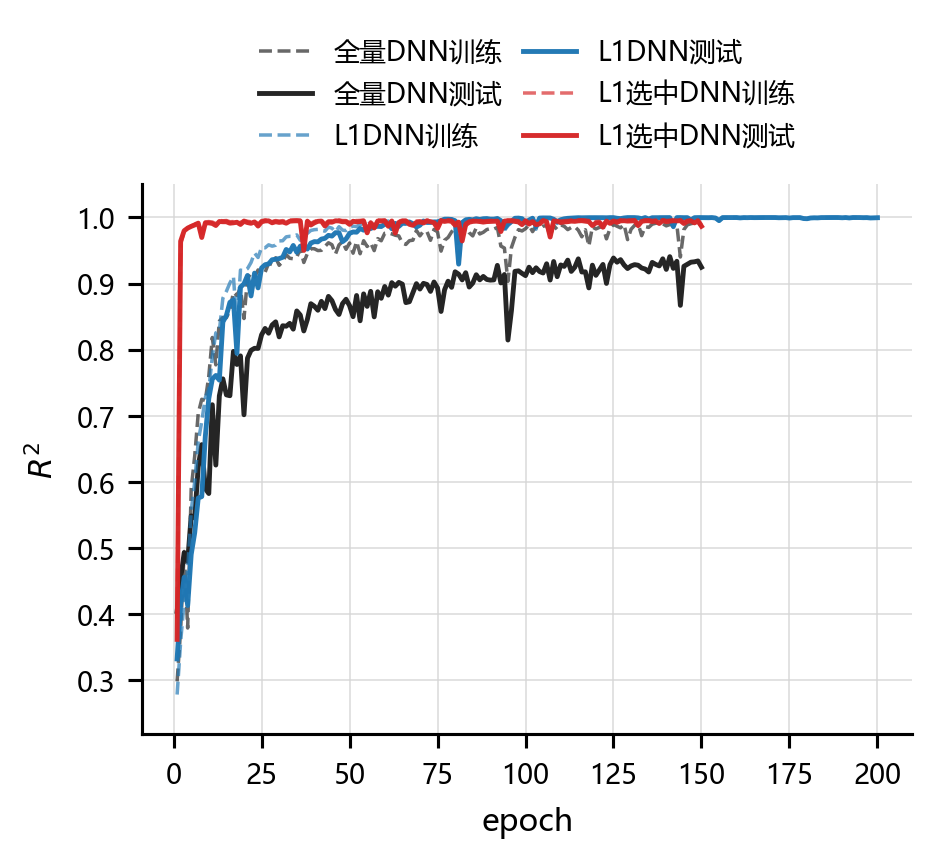
\includegraphics[width=\columnwidth]{redundant_training_congestion_zh.png}\\[-0.2em]
{\scriptsize (a) 日前拥塞价}\\[0.45em]
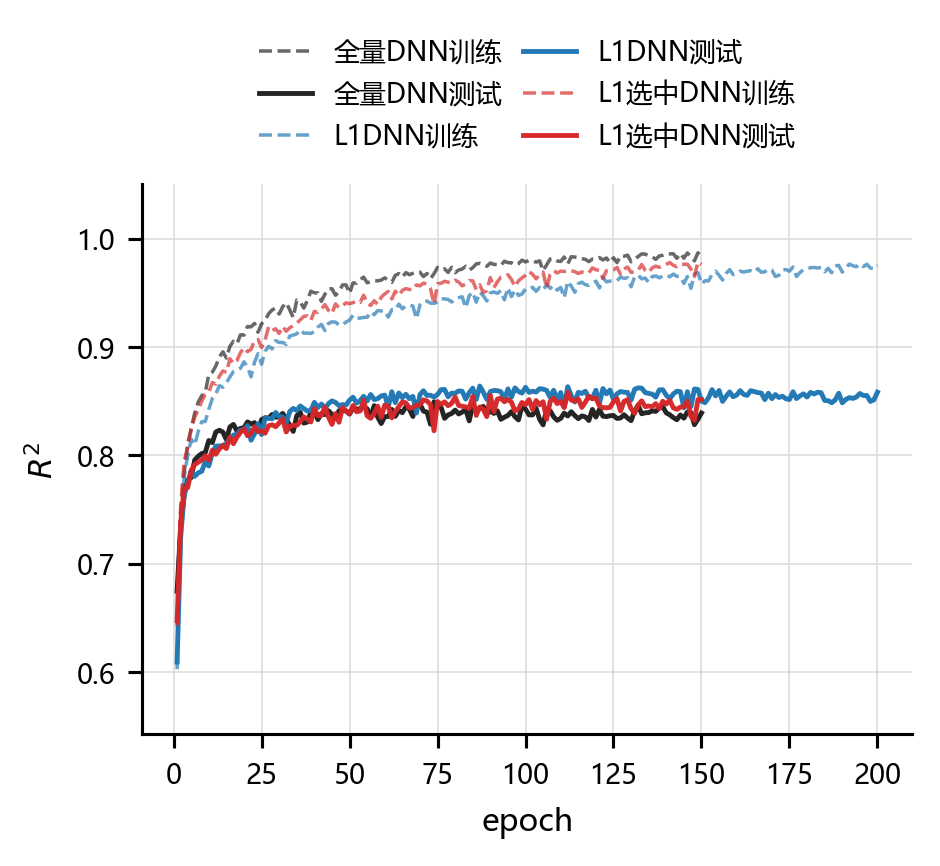
\includegraphics[width=\columnwidth]{redundant_training_primary_zh.png}\\[-0.2em]
{\scriptsize (b) 主备用容量}
\figbicaption{全量字段与 L1 选中特征的训练/测试 $R^2$ 曲线对比}{Comparison of train/test $R^2$ curves between all features and L1-selected features}
\label{fig:redundant_curve}
\end{figure}

\begin{table}[!htbp]
\centering
\scriptsize
\setlength{\tabcolsep}{3pt}
\tabbicaption{冗余信息影响分析的训练曲线统计}{Training-curve statistics for redundant-information analysis}
\label{tab:noise_curve}
\textbf{(a) 日前拥塞价}\\[-0.2em]
\begin{tabularx}{\columnwidth}{Xrrrr}
\toprule
方法 & 字段数 & Best $R^2$ & epoch & 泛化差距 \\
\midrule
全量 DNN & 69 & 0.9408 & 141 & 0.0621 \\
L1GateDNN & 69 & 1.0000 & 194 & -0.0001 \\
L1 选中特征 DNN & 2 & 0.9954 & 139 & 0.0025 \\
\bottomrule
\end{tabularx}

\vspace{0.4em}
\textbf{(b) 主备用容量}\\[-0.2em]
\begin{tabularx}{\columnwidth}{Xrrrr}
\toprule
方法 & 字段数 & Best $R^2$ & epoch & 泛化差距 \\
\midrule
全量 DNN & 69 & 0.8495 & 74 & 0.1439 \\
L1GateDNN & 69 & 0.8639 & 87 & 0.1170 \\
L1 选中特征 DNN & 35 & 0.8580 & 112 & 0.1247 \\
\bottomrule
\end{tabularx}
\end{table}

\subsubsection{Top-n 递增实验}
为进一步揭示字段数量与推断性能之间的关系，本文按 L1 门控值排名逐步增加输入字段数，记录各组合下的测试 $R^2$。图~\ref{fig:topn_noise} 给出了日前拥塞价和主备用容量两个目标的完整 Top-n 序列结果，其中三角形标记表示 $R^2$ 最高点，方形标记表示全量字段对应的结果。

日前拥塞价目标上，Top2 即达 0.9954、Top3 升至 0.9999，并在 Top24 内保持高位，而增至 Top32 时回落到 0.9851，全量 69 字段仅 0.9408；主备用容量目标上，$R^2$ 在 Top24 达到 0.8872 的峰值后，于 Top32、Top35 回落至约 0.854，接近全量 DNN 的 0.8495。

递增实验揭示了字段数量与推断性能间的非单调关系：关键字段不足时能力受限，字段数适中时核心路径被充分激活而精度显著提升，冗余字段继续加入则因维度增大、过拟合上升导致泛化收益递减甚至逆转。这表明适度压缩字段不仅不损害推断能力，反而可能因消除冗余而改善泛化。

\begin{figure}[!htbp]
\centering
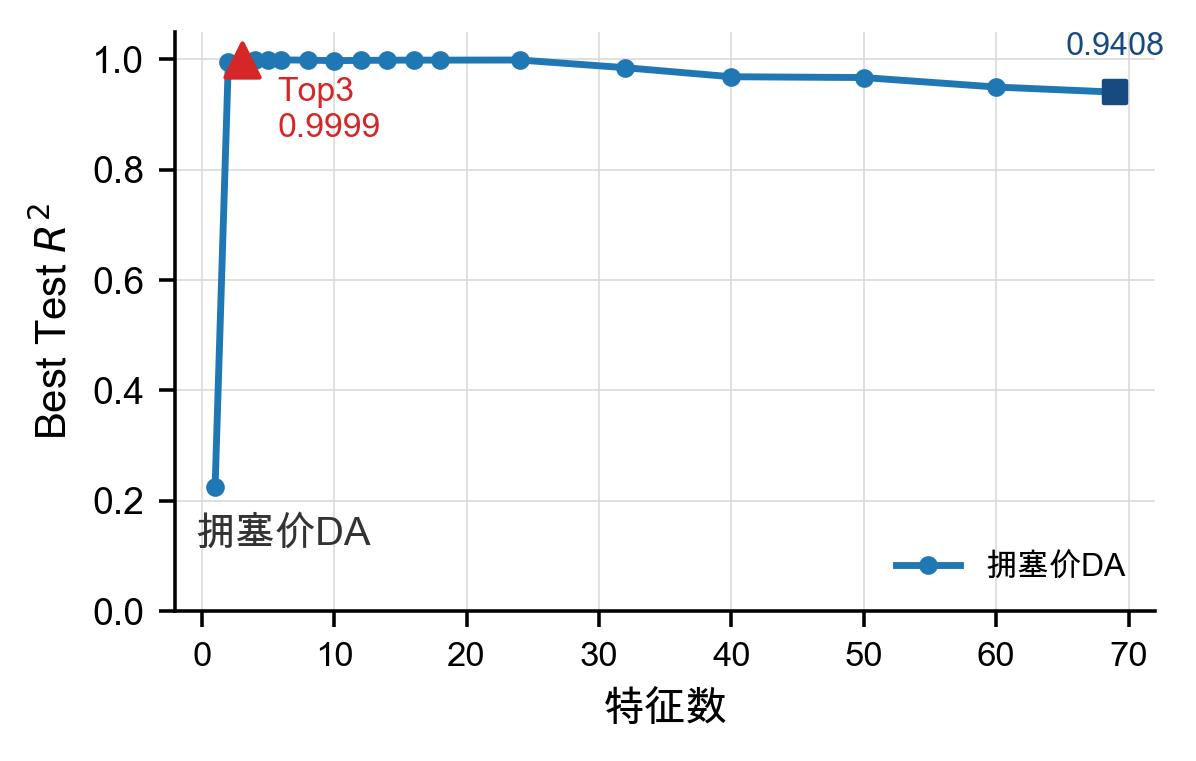
\includegraphics[width=\columnwidth]{topn_congestion_zh.png}\\[-0.2em]
{\scriptsize (a) 日前拥塞价}\\[0.45em]
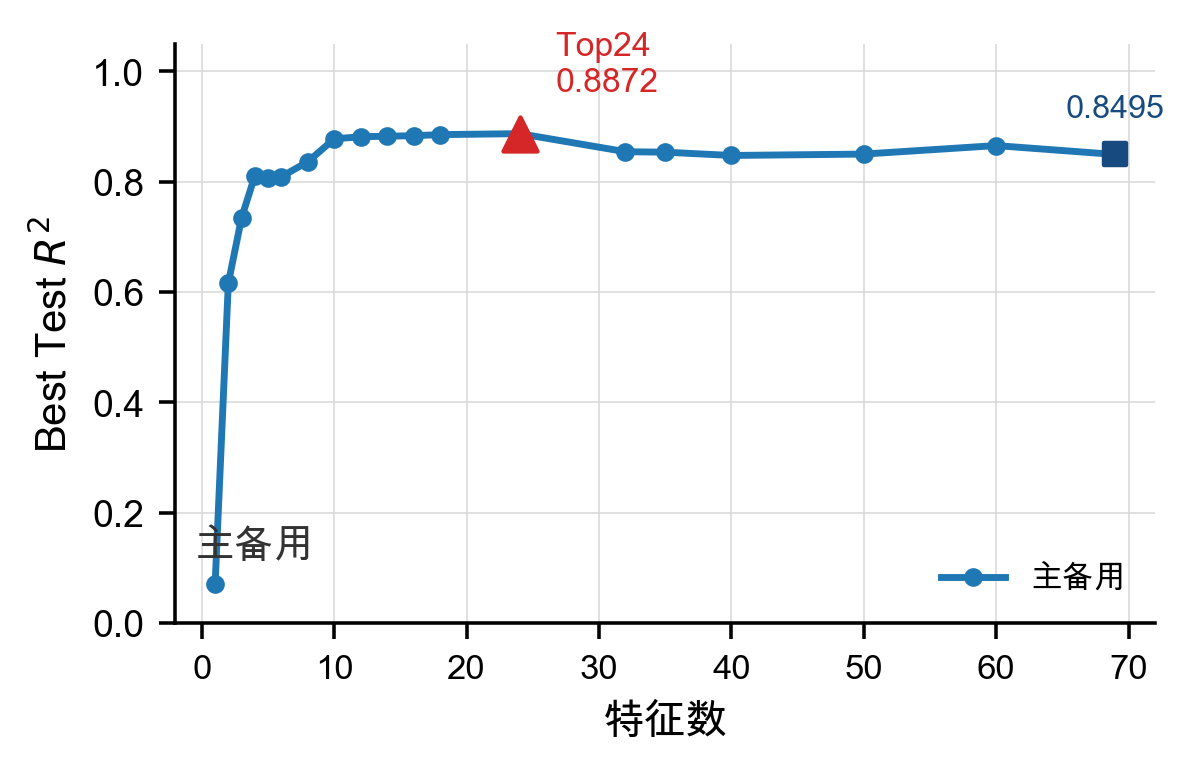
\includegraphics[width=\columnwidth]{topn_primary_zh.png}\\[-0.2em]
{\scriptsize (b) 主备用容量}
\figbicaption{按 L1 门控排名逐步增加字段数的测试 $R^2$ 变化}{Test $R^2$ variation with incrementally added Top-n features ranked by L1 gate values}
\label{fig:topn_noise}
\end{figure}

\section{结论}
本文围绕电力数据关联分析中的隐性推断源定位问题，提出一种融合多相关性筛选与 L1 门控深度神经网络的方法。该方法先以六类统计指标对候选字段进行多维依赖性初筛，确保不同类型的潜在推断源字段均被保留；再以 L1 门控 DNN 在保持目标推断能力的前提下自动压缩冗余字段，获取紧凑的推断源集合，并通过普通 DNN 再训练加以独立验证；进而构建相关性驱动的改进门控，使各类相关性指标对推断贡献的权重由数据自动学习，增强了方法的可解释性。

基于 PJM 2025 年小时级运行数据的实验表明：针对净实际交换功率，所提方法从 69 个候选字段中定位出 18 个推断源，再训练 DNN 的测试 $R^2$ 为 0.9681，高于全量字段的 0.9661，而其余 51 个字段单独推断仅为 0.7820；在 12 个目标字段上，方法以平均 15.5 个字段（约占全量的 22.46\%）取得 0.9111 的平均 $R^2$，优于全量 DNN 的 0.9031；同预算对比中其平均 $R^2$ 在各预算水平下均保持领先。冗余信息分析进一步揭示了全量输入中弱相关字段引发过拟合的机理，为字段压缩策略提供了实证依据。总体而言，所提方法能够有效定位电力数据中的关键推断源字段，可为数据共享前的字段关联性审查、字段价值评估与推断路径分析提供支撑。

本文方法仍有可拓展之处：一方面，部分目标字段可能存在多条等价推断路径，单次训练得到的推断源集合不一定唯一，后续可引入多随机种子与跨时间窗口验证评估其稳定性，并将单目标分析扩展为刻画字段间联合推断关系的多目标关联图谱；另一方面，可将所定位的推断源集合与字段降精度、延迟发布、分级共享等数据处置策略\cite{ref-zhu-sharing}相结合，构建面向实际电力数据共享流程的闭环分析机制。

\balance
\begin{thebibliography}{99}
\bibitem{ref-liu-cps}
刘涛, 田捷, 王杰, 等. 信息物理融合系统的综合安全威胁与防御研究[J]. 自动化学报, 2019, 45(1): 5-24.

LIU Tao, TIAN Jie, WANG Jie, et al. Integrated security threats and defense of cyber-physical systems[J]. Acta Automatica Sinica, 2019, 45(1): 5-24.

\bibitem{ref-ma-pjm}
马珍, 张弘, 朱兰, 等. 美国电力市场信息披露制度及其对中国的启示[J]. 电力系统自动化, 2017, 41(24): 49-57.

MA Zhen, ZHANG Hong, ZHU Lan, et al. Information disclosure system in American electricity market and its enlightenment for China[J]. Automation of Electric Power Systems, 2017, 41(24): 49-57.

\bibitem{ref-fan-pjm}
Fan Z, Horger T, Bastian J, et al. An overview of PJM energy market design and development[C]//2008 Third International Conference on Electric Utility Deregulation and Restructuring and Power Technologies. Piscataway: IEEE, 2008: 12-17.

\bibitem{ref-xing-micdnn}
邢治, 王征, 冯健, 等. MIC-DNN：电力数据关联分析框架[C]//2025 40th Youth Academic Annual Conference of Chinese Association of Automation. Piscataway: IEEE, 2025: 2969-2974.

XING Zhi, WANG Zheng, FENG Jian, et al. MIC-DNN: Data-driven correlation analysis framework for power data[C]//2025 40th Youth Academic Annual Conference of Chinese Association of Automation. Piscataway: IEEE, 2025: 2969-2974.

\bibitem{ref-liu-inference}
刘烃, 王子骏, 刘杨, 等. 数据推断：信息物理融合系统数据泄露威胁范式和防御方法[J]. 中国科学：信息科学, 2023, 53(11): 2152-2179.

LIU Ting, WANG Zijun, LIU Yang, et al. Data inference: A paradigm of data leakage threats and defense methods for cyber-physical systems[J]. Scientia Sinica Informationis, 2023, 53(11): 2152-2179.

\bibitem{ref-sankar}
Sankar L, Rajagopalan S R, Mohajer S, et al. Smart meter privacy: A theoretical framework[J]. IEEE Transactions on Smart Grid, 2013, 4(2): 837-846.

\bibitem{ref-giaconi}
Giaconi G, Gündüz D, Poor H V. Privacy-aware smart metering: Progress and challenges[J]. IEEE Signal Processing Magazine, 2018, 35(6): 59-78.

\bibitem{ref-adewole}
Adewole K S, Torra V. Privacy issues in smart grid data: From energy disaggregation to disclosure risk[C]//International Conference on Database and Expert Systems Applications. Cham: Springer, 2022: 71-84.

\bibitem{ref-chen-privacy}
陈颖, 王科, 朱涛, 等. 电力大数据隐私保护技术综述[J]. 电力系统自动化, 2021, 45(14): 157-168.

CHEN Ying, WANG Ke, ZHU Tao, et al. Review on privacy-preserving technologies for power big data[J]. Automation of Electric Power Systems, 2021, 45(14): 157-168.

\bibitem{ref-zhang-sgcc}
张伯明, 孙宏斌, 吴文传, 等. 智能电网控制中心的信息安全问题[J]. 南方电网技术, 2012, 6(2): 1-7.

ZHANG Boming, SUN Hongbin, WU Wenchuan, et al. Information security issues in smart grid control centers[J]. Southern Power System Technology, 2012, 6(2): 1-7.

\bibitem{ref-deng-load}
邓鑫, 张超, 彭辉, 等. 基于相关性分析与特征提取的区域电网短期负荷预测[C]//2022 7th Asia Conference on Power and Electrical Engineering. Piscataway: IEEE, 2022: 1081-1085.

DENG Xin, ZHANG Chao, PENG Hui, et al. Short-term load forecasting for regional power grids based on correlation analysis and feature extraction[C]//2022 7th Asia Conference on Power and Electrical Engineering. Piscataway: IEEE, 2022: 1081-1085.

\bibitem{ref-lan-load}
兰丁, 朱慧, 吴杰, 等. 基于改进 AlexNet-GRU 深度学习网络的配电网短期负荷预测方法[C]//2021 IEEE 5th Conference on Energy Internet and Energy System Integration. Piscataway: IEEE, 2021: 3004-3010.

LAN Ding, ZHU Hui, WU Jie, et al. A short-term load forecasting method of distribution network based on improved AlexNet-GRU deep learning network[C]//2021 IEEE 5th Conference on Energy Internet and Energy System Integration. Piscataway: IEEE, 2021: 3004-3010.

\bibitem{ref-jiao-pv}
焦鑫, 孙源, 彭迪, 等. 基于方差变点与相关性分析的光伏功率异常数据清洗[C]//2021 6th International Conference on Power and Renewable Energy. Piscataway: IEEE, 2021: 1140-1145.

JIAO Xin, SUN Yuan, PENG Di, et al. Photovoltaic power abnormal data cleaning based on variance change point and correlation analysis[C]//2021 6th International Conference on Power and Renewable Energy. Piscataway: IEEE, 2021: 1140-1145.

\bibitem{ref-szekely-dcorr}
Székely G J, Rizzo M L, Bakirov N K. Measuring and testing dependence by correlation of distances[J]. The Annals of Statistics, 2007, 35(6): 2769-2794.

\bibitem{ref-gretton-hsic}
Gretton A, Bousquet O, Smola A, et al. Measuring statistical dependence with Hilbert-Schmidt norms[C]//Algorithmic Learning Theory. Berlin: Springer, 2005: 63-77.

\bibitem{ref-reshef-mic}
Reshef D N, Reshef Y A, Finucane H K, et al. Detecting novel associations in large data sets[J]. Science, 2011, 334(6062): 1518-1524.

\bibitem{ref-lecun-deep}
LeCun Y, Bengio Y, Hinton G. Deep learning[J]. Nature, 2015, 521(7553): 436-444.

\bibitem{ref-goodfellow-deep}
Goodfellow I, Bengio Y, Courville A. Deep learning[M]. Cambridge: MIT Press, 2016.

\bibitem{ref-breiman-rf}
Breiman L. Random forests[J]. Machine Learning, 2001, 45(1): 5-32.

\bibitem{ref-chen-xgboost}
Chen T, Guestrin C. XGBoost: A scalable tree boosting system[C]//Proceedings of the 22nd ACM SIGKDD International Conference on Knowledge Discovery and Data Mining. New York: ACM, 2016: 785-794.

\bibitem{ref-wang-meter}
Wang Y, Chen Q, Hong T, et al. Review of smart meter data analytics: Applications, methodologies, and challenges[J]. IEEE Transactions on Smart Grid, 2019, 10(3): 3125-3148.

\bibitem{ref-tibshirani-lasso}
Tibshirani R. Regression shrinkage and selection via the lasso[J]. Journal of the Royal Statistical Society: Series B, 1996, 58(1): 267-288.

\bibitem{ref-zou-enet}
Zou H, Hastie T. Regularization and variable selection via the elastic net[J]. Journal of the Royal Statistical Society: Series B, 2005, 67(2): 301-320.

\bibitem{ref-cover-info}
Cover T M, Thomas J A. Elements of information theory[M]. 2nd ed. Hoboken: John Wiley \& Sons, 2006.

\bibitem{ref-pjm-dataminer}
PJM Interconnection. PJM Data Miner 2[EB/OL]. [2025-05-01]. https://dataminer2.pjm.com.

\bibitem{ref-kingma-adam}
Kingma D P, Ba J. Adam: A method for stochastic optimization[C]//International Conference on Learning Representations. San Diego: ICLR, 2015.

\bibitem{ref-he-dropout}
Srivastava N, Hinton G, Krizhevsky A, et al. Dropout: A simple way to prevent neural networks from overfitting[J]. The Journal of Machine Learning Research, 2014, 15(1): 1929-1958.

\bibitem{ref-zhu-sharing}
朱涛, 陈颖, 张宁, 等. 面向电力数据共享的安全机制研究[J]. 中国电机工程学报, 2020, 40(S1): 21-30.

ZHU Tao, CHEN Ying, ZHANG Ning, et al. Security mechanisms for power data sharing[J]. Proceedings of the CSEE, 2020, 40(S1): 21-30.
\end{thebibliography}

\section*{收稿日期与作者简介}
\noindent\textbf{收稿日期：}20XX-XX-XX

\noindent\textbf{作者简介：}\par
\noindent 杜浩存（出生年），男，研究方向为电力数据关联分析、信息物理系统安全与机器学习，邮箱：待补充。

\end{document}
